
% !TEX root = ../Testa/Principale.tex
% LTeX: language=it

\chapter{Note di teoria dei grafi}\label{secTeoriaGrafi}

    In questo capitolo sono prima introdotti alcuni oggetti di base della teoria dei grafi, quindi si discute la natura della rete d'interesse, infine si descriveranno molto brevemente i dati usati.

    \section{Definizioni miscellanee}\label{secDefinizioniGrafi}

        Innanzitutto s'inizia dando la definizione di rete:
        
        \begin{dfn}[Grafo]
            \label{defGrafo}
            Un grafo è formato dalla coppia \(\mathcal G=(\mathcal I,\mathcal E)\), ove \(\mathcal I\) è l'insieme degl'indici dei nodi mentre \(\mathcal I\) è l'insieme dei lati, vale a dire di coppie d'indici \(\mathcal I\): due nodi \(i,j\in\mathcal I\) sono connessi sse \((i,j)\in\mathcal E\).
        \end{dfn}
        
        Dall'insieme \(\mathcal E\) si può poi specializzare il concetto di grafo:
        
        \begin{dfn}[Grafo \textnormal{[in]}diretto]
            \label{defGrafoInDiretto}
            Un grafo è indiretto sse dato \((i,j)\in\mathcal E\) allora \((j,i)\in\mathcal E\) e la direzione è trascurabile; altrimenti è detto diretto.
        \end{dfn}
        
        La trascurabilità della direzione sarà discussa poco dopo nella \cref{secRetiECittà}, anche se è facilmente intuibile dalla \cref{figEsempioGrafoInDiretto}.

        \tikzfigure{H}
            {
% !TEX root = ../../../Esperimenti/.tex/MEF.tex
% LTeX: language=it

\begin{tikzpicture}[%
    node distance=5em,
    main node/.style={
        circle,
        draw,
        thick,
        fill=white,
        inner sep=0pt,
        minimum size=1.25em
    }, % Ponendo la separazione interna nulla la dimensione del cerchio sarà data dalla chiave «minimum size», oltre che dalla dimensione del testo stesso
    edge/.style={thick}
]
    % \renewcommand\subCaptionSize{10}

    \pgfmathsetmacro\radius{1.5}
    \newcommand\hSepPlot{10em}
    \newcommand\hSepLabel{1.5em}

    % Grafo Indiretto a forma di triangolo equilatero
    \node[main node] (A) at (90:\radius) {1};
    \node[main node] (B) at (330:\radius) {2};
    \node[main node] (C) at (210:\radius) {3};
    % Coordinate polari: (angolo:raggio)

    \draw[edge] (A) -- (B);
    \draw[edge] (B) -- (C);
    \draw[edge] (C) -- (A);

    \node[left=\hSepLabel of A] {\dimTesto{\subCaptionSize}\sottoDidascalia[]{}};
    % \node[below=\hSepLabel of 1] {\textbf{Grafo Indiretto}};
    
    % Grado diretto a forma di triangolo equilatero
    \begin{scope}[xshift=\hSepPlot]
        \node[main node] (A) at (90:\radius) {1};
        \node[main node] (B) at (330:\radius) {2};
        \node[main node] (C) at (210:\radius) {3};

        \draw[edge, -{Stealth}] (A) edge[bend left=15] (B);
        \draw[edge, -{Stealth}] (B) edge[bend left=15] (A);

        \draw[edge, -{Stealth}] (B) edge[bend left=15] (C);
        \draw[edge, -{Stealth}] (C) edge[bend left=15] (B);

        \draw[edge, -{Stealth}] (C) edge[bend left=15] (A);
        \draw[edge, -{Stealth}] (A) edge[bend left=15] (C);

        \node[left=\hSepLabel of A] {\dimTesto{\subCaptionSize}\sottoDidascalia[]{}};
        % \node[below=\hSepLabel of A] {\textbf{Grafo Diretto Simmetrico}};
    \end{scope}

    % Matrice d'adiacenza
    \pgfmathparse{1.9*\hSepPlot}
    \begin{scope}[xshift=\pgfmathresult]
        \node[
            inner sep=0pt,
            outer sep=0pt
        ] (M) {
            \(
                A = 
                \begin{bmatrix}
                    0 & 1 & 1 \\
                    1 & 0 & 1 \\
                    1 & 1 & 0 
                \end{bmatrix}%
            \)%
        };%

        \node at (90:\radius) {\dimTesto{\subCaptionSize}\sottoDidascalia[]{}};
        % \pgfmathparse{\radius/sqrt(3)}
        % \node[above=\pgfmathresult em of M] {\sottoDidascalia[]{}};
    \end{scope}%
\end{tikzpicture}%}
            {Esempio di un grafo indiretto, della sua equivalente forma diretta [simmetrica] e della loro [identica] matrice d'adiacenza.}
            {.9\linewidth}{figEsempioGrafoInDiretto}
        
        \begin{dfn}[Matrice d'adiacenza]
            \label{defMatriceAdiacenzaUnitariaPesata}
            \newcommand\hspz{\hspace{1em}}
            Sia \(N\equiv\vert\mathcal I\vert\in\NPlus\) la cardinalità dell'insieme degl'indici, ossia il numero di vertici totali, si definisce la matrice d'adiacenza \(\mathbf M\in\mathbb R^{N\times N}\) pesata come:
            %
            \begin{equation}
                \label{eqMatriceAdiacenzaPesata}
                m_{i,j}\equiv
                \left\{\begin{aligned}
                    q_{i,j}&\hspz\text{ se }(i,j)\in\mathcal E,\\
                    0&\hspz\text{ altrimenti},
                \end{aligned}\right.
            \end{equation}
            %
            ove \(q_{i,j}\in\mathbb R\) è il peso associato al lato \((i,j)\); nel caso in cui \(q_{i,j}\equiv1\) \(\forall i,j\in\mathcal I\) si ha la matrice d'adiacenza unitaria \(\mathbf A\in\mathbb R^{N\times N}\):
            %
            \begin{equation}
                \label{eqMatriceAdiacenzaUnitaria}
                a_{i,j}\equiv
                \left\{\begin{aligned}
                    1&\hspz\text{ se }(i,j)\in\mathcal E,\\
                    0&\hspz\text{ altrimenti}.
                \end{aligned}\right.
            \end{equation}
            %
            Si osserva che, se non altrimenti detto, scrivendo solo «matrice d'adiacenza» si sottintende sempre quella unitaria.
        \end{dfn}

        \begin{dfn}[Matrice trasposta]
            Data \(\mathbf M\in\mathbb R^{N\times N}\), con \(N\in\NPlus\), allora s'indica \(\mathbf M^\top\) la matrice trasposta cosí definita:
            %
            \begin{equation*}
                m^\top_{i,j}=m_{j,i}\quad\forall i,j\in\{1,2,\ldots,N\}.
            \end{equation*}
        \end{dfn}

        \begin{dfn}[Matrice simmetrica]
            Data \(\mathbf M\in\mathbb R^{N\times N}\), con \(N\in\NPlus\), allora
            %
            \begin{equation}
                \label{eqMatriceAdiacenzaSimmetrica}
                \mathbf M\text{ è simmetrica}
                \ \ \iff\ \ 
                m_{i,j}=m_{j,i}=m^\top_{i,j}
                \ \ \iff\ \ 
                \mathbf M=\mathbf M^\top.
            \end{equation}
        \end{dfn}

        \begin{oss}
            Nei grafi indiretti sia \(\mathbf M\) che \(\mathbf A\) sono simmetriche mentre per quelli diretti non è detto lo siano.
        \end{oss}

        \begin{dfn}[Gradi e Forze]
            \label{defForzaGradoEntranteUscente}
            In un grafo diretto e pesato si definiscono la forza entrante e uscente come rispettivamente le quantità
            %
            \begin{equation}
                \label{eqForzaGrafoDiretto}
                w^-_i\equiv\sum_{j=1}^{\vert\mathcal I\vert}m_{j,i}%=(\mathbf M^\top\mathbf 1)_i
                \quad\text{e}\quad
                w^+_i\equiv\sum_{j=1}^{\vert\mathcal I\vert}m_{i,j},%=(\mathbf M\mathbf 1)_i,
                \quad\forall i\in\mathcal I,
            \end{equation}
            %
            % dove \(\mathbf 1\equiv(1,1,\ldots,1)\in\mathbb R^N\);
            le quali se il grafo è simmetrico queste coincidono: \(\mathbf w=\mathbf w^-=\mathbf w^+\). Nel caso unitario \(\mathbf M\equiv\mathbf A\) si è soliti denominare le forze come gradi uscenti ed entranti:
            %
            \begin{equation}
                \label{eqGradoGrafoDiretto}
                k^-_i\equiv\sum_{j=1}^{\vert\mathcal I\vert}a_{j,i}%=(\mathbf A^\top\mathbf 1)_i
                \quad\text{e}\quad
                k^+_i\equiv\sum_{j=1}^{\vert\mathcal I\vert}a_{i,j},%=(\mathbf A\mathbf 1)_i,
                \quad\forall i\in\mathcal I,
            \end{equation}
            %
            che, come prima, in una rete simmetrica coincidono: \(\mathbf k=\mathbf k^-=\mathbf k^+\).
        \end{dfn}

    \section{Reti e città}\label{secRetiECittà}

        Dopo aver illustrato un po' di teoria sui grafi sorge successivamente il problema di come rappresentare con essi la moltitudine di collegamenti possibili tra le città
        
        Difatti vi sono molti modi di rappresentare le città mediante i grafi: i primi si pongono a livello \textit{intraurbano}, o considerando le strade come lati e le loro intersezioni come nodi \cite[§ 3.1.3.1 p. 17]{Barthelemy2011}, o rappresentando la rete di trasporto di tram, di bus e della metro \cite[§ 3.2.1 p. 22]{Barthelemy2011}; altri si pongono piú propriamente a livello \textit{interurbano} prendono singolarmente in considerazione varie reti dei trasporti (ferroviario \cite[§ 3.1.3.2 p. 17]{Barthelemy2011}, navale \cite[§ 3.1.4 p. 19]{Barthelemy2011}, aereo \cite[§ 3.1.2 p. 13]{Barthelemy2011}, ecc.).

        Tuttavia, da quanto detto nella \cref{secIntroduzione}, è chiaro che per predire la distribuzione della popolazione tra città valgono le seguenti osservazioni:

        \begin{enumerate}[
            label=\arabic*.,
            topsep=0.5em,
            parsep=0em,
            itemsep=0.25em,
            leftmargin=2em,
            rightmargin=1.5em,
            % \leftmargin + \itemindent = \labelindent + \labelwidth + \labelsep
            %itemindent=!,
            %labelindent=3em,
            %labelwidth=!,
            %labelsep=!,
        ]
            \item ogni rappresentazione intraurbana va scartata perché sono troppo fini, oltre a considerare movimenti limitatamente a una sola città;
            \item d'altra parte tutte quelle interurbane vanno considerate contemporaneamente e non singolarmente siccome ciascun individuo può scegliere diversi trasporti per muoversi.
        \end{enumerate}

        Ecco perché la corretta rete da considerare è quella legata ai movimenti pendolari \bracketcitesemi[§ 3.1.3.3 p. 18]{Barthelemy2011}[]{DeMontis2007} tra città che mostrano olisticamente tutt'i possibili collegamenti tra le città a prescindere del trasporto scelto; inoltre essa mostra collegamenti realistici associati a movimenti quotidiani anziché straordinari (vacanze, visite mediche, ecc.).

        Una volta fissata la rappresentazione è necessario comprendere il tipo di grafo con cui si ha a che fare. Eppure qui la risposta è immediata dopo due osservazioni:
       
        \begin{enumerate}[
            label=\arabic*.,
            topsep=0.5em,
            parsep=0em,
            itemsep=0.25em,
            leftmargin=2em,
            rightmargin=1.5em,
            % \leftmargin + \itemindent = \labelindent + \labelwidth + \labelsep
            %itemindent=!,
            %labelindent=3em,
            %labelwidth=!,
            %labelsep=!,
        ]
            \item una città può interagire con un'altra senza che quest'ultima interagisca colla prima: è necessario considerare il senso di direzione;
            \item ammesso che una città possa interagire con un'altra, allora è sempre possibile l'opposta: le potenziali interazioni sono simmetriche.
        \end{enumerate}
    
        Dunque il grafo in questione è diretto ma con struttura indiretta (\cref{defGrafoInDiretto}), ovvero la sua matrice d'adiacenza \(\mathbf A\) è simmetrica.

        \begin{ipo}
            \label{ipTipoGrafo}
            Il grafo \(\mathcal G\) è diretto e simmetrico (\(\mathbf A\) è simmetrica).
        \end{ipo}

        Inoltre in questa trattazione vale la seguente fondamentale ipotesi:

        \begin{ipo}
            \label{ipGrafoStatico}
            Il grafo \(\mathcal G\) è statico: \(\mathcal I\) e \(\mathcal E\) sono costanti nel tempo.
        \end{ipo}

        In altre parole si è solo interessati a prevedere come la popolazione si distribuisce rispetto a una topologia prestabilita \textit{a priori}; ovviamente si tratta di una forte semplificazione dato che nella realtà la topologia delle connessioni interurbane si è chiaramente coevoluta assieme allo sviluppo delle città stesse.

        Infine si osserva che questo tipo di grafo è spaziale \cite{Barthelemy2011,DeMontis2007}, ovvero i suoi nodi occupano un punto nello spazio euclideo, seppure, al momento, sia una caratteristica alquanto formale; tuttavia servirà tenerlo a mente quando si definiranno alcune regole d'interazione nel \cref{secSimulazioni}. Perdipiú, contrariamente a quanto si possa pensare di primo acchito, tale grafo non è a invarianza di scala \cite{Barabasi1999} a causa del tipo di grafo \cite{Broido2019,Barthelemy2011}; ciò non esclude l'esistenza di nodi piú centrali di altri, ma solo che il massimo grado di un nodo è limitato superiormente proprio dalla natura spaziale del grafo.

    \section{Cenni sui dati}\label{secCenniSuiDati}

        La matrice di pendolarismo costruita è quella fornita dall'ISTAT del 1991 \cite{ISTATPendolarismo1991} seguendo l'esempio di \cite{DeMontis2007}. I dati sono di fatto un \textit{file} di testo formato da una serie di righe di 29 numeri il cui significato è spiegato dalla \cref{tabStrutturaDatiPendolarismo}.

        \begin{table}[htb]
            \centering
            \begin{NiceTabular}{ccc}
                % \CodeBefore
                %     \chessboardcolors{red!15}{blue!15}
                % \Body
                    \hline
                    Dato & Col. iniziale & Lunghezza \\
                    \hline
                    Provincia di partenza & 1 & 3 \\
                    Comune di partenza & 4 & 3 \\
                    Sesso & 7 & 1 \\
                    Mezzo di trasporto & 8 & 1 \\
                    Cond.professionale & 9 & 1 \\
                    Orario di uscita & 10 & 1 \\
                    Tempo di percorrenza & 11 & 1 \\
                    Provincia di arrivo & 12 & 3 \\
                    Comune di arrivo & 15 & 3 \\
                    Numero di persone & 18 & 12 \\
                    \hline
                \CodeAfter
                    \tikz \foreach \r in {4,...,8} \draw (\r.5-|1) -- (\r.5-|4);
            \end{NiceTabular}
            \captionsetup{width=.75\textwidth}
            \caption{Formattazione di una sola riga nei dati ISTAT\protect\footnotemark; le linee barrate corrispondono a dati trascurati.}
            \label{tabStrutturaDatiPendolarismo}
        \end{table}
        \footnotetext{si v. il documento \texttt{trapen91.txt} per maggiori informazioni.}

        I comuni considerati sono tutt'i quell'italiani (8100) nel 1991, quindi è necessario estrapolare da essi le matrici di pendolarismo delle singole regioni e parallelamente quella complessiva dell'Italia. Si possono definire due tipi di matrici:

        \begin{enumerate}[
            label=\arabic*.,
            topsep=0.5em,
            parsep=0em,
            itemsep=0.25em,
            leftmargin=2em,
            rightmargin=1.5em,
            % \leftmargin + \itemindent = \labelindent + \labelwidth + \labelsep
            %itemindent=!,
            %labelindent=3em,
            %labelwidth=!,
            %labelsep=!,
        ]
            \item quella d'adiacenza unitaria in cui un lato esiste se almeno un pendolare (cioè il «[n]umero di persone» nella \cref{tabStrutturaDatiPendolarismo}) si muove tra i due comuni e
            \item quella d'adiacenza pesata che è analoga alla precedente ma con peso \(q_{i,j}\) uguale alla somma totale dei pendolari tra due comuni.
        \end{enumerate}

        Si notano tuttavia due principali difetti dei dati contenuti nel documento \texttt{Pen\_91It.txt}:

        \begin{enumerate}[
            label=\arabic*.,
            topsep=0.5em,
            parsep=0em,
            itemsep=0.25em,
            leftmargin=2em,
            rightmargin=1.5em,
            % \leftmargin + \itemindent = \labelindent + \labelwidth + \labelsep
            %itemindent=!,
            %labelindent=3em,
            %labelwidth=!,
            %labelsep=!,
        ]
            \item in alcune linee come comune di destinazione è segnato il codice «022008» che però non è elencato nel documento \texttt{elencom91.xls} che riassume tutti gli 8100 comuni italiani nel 1991;
            \item in molte linee come comune di destinazione sono segnati dei codici incompleti contenenti solo l'ultima metà (codice comune) ma non la prima (codice provincia), e questi sono in totale 8: «215», «229», «241», «216», «203», «224», «236», «246».
        \end{enumerate}

        In entrambi i casi i dati relativi [a quelli che sono potenzialmente refusi] sono stati trascurati nella corrente tesi; il primo errore è già di per sé molto raro, mentre il secondo è eccessivamente ambiguo da risolvere come si può notare dalla linea successiva relativa al codice «215»:
        %
        \begin{center}
            \texttt{00200714212215\_\_\_\_\_\_\_\_\_\_\_\_\_\_1},
        \end{center}
        %
        ove \_ indica uno spazio, per la quale, tralasciando il fatto che vi sono in totale 6 città italiane collo stesso codice comunale, se ci si limita alla regione del Piemonte (vale a dire la stessa del comune di partenza «002007») esistono in realtà ben due città condividenti lo stesso codice: «001215» e «004215», eppure entrambe non hanno lo stesso codice provinciale («002») del comune di partenza. Da questo piccolo estratto, quindi, non si può nemmeno ipotizzare che il codice provinciale sia lo stesso tra il comune di partenza e d'arrivo; è allora chiaro che sia impossibile scegliere la prima metà per completare il codice del comune di destinazione.

        \begin{oss}
            A dire il vero si potrebbe scegliere, tra tutt'i comuni collo stesso codice comunale, quello che minimizza la distanza geografica (ossia euleriana) siccome le coordinate dei punti rappresentativi di ogni comune sono disponibili nell'ISTAT \cite{ISTATLimiti1991}. In ogni caso il numero cosí esiguo d'eccezioni rendono una tale "correzione" del tutto innecessaria, oltre che irrilevante come il \cref{secSimulazioni} mostrerà.
        \end{oss}

        \tikzfigure{H}
            {% This file was created by matlab2tikz.
%

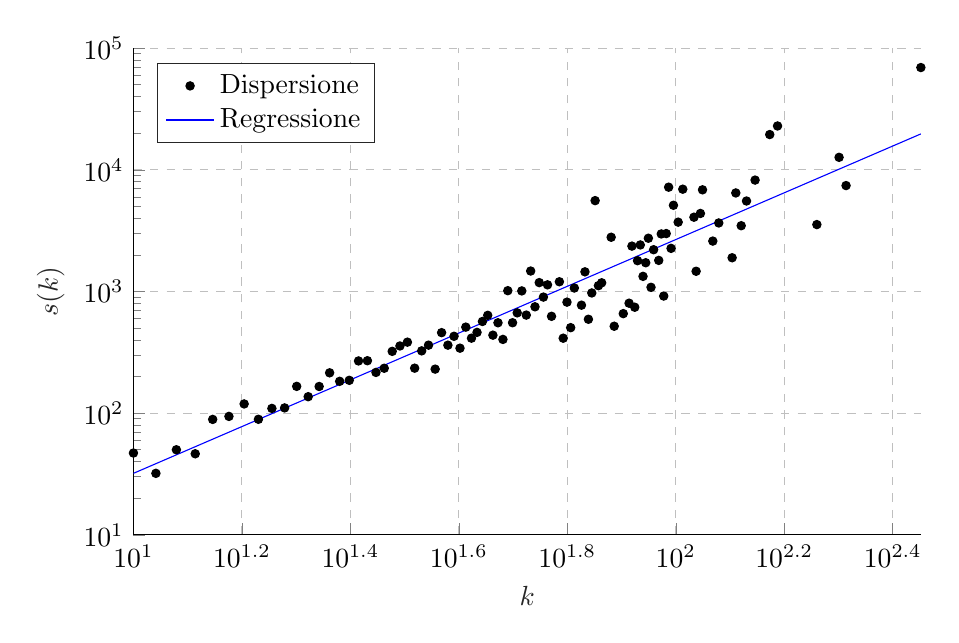
\begin{tikzpicture}
    \definecolor{mycolor1}{rgb}{0.00000,0.44700,0.74100}%
    %
    \pgfmathsetlengthmacro\plotWidth{10cm}
    \pgfmathsetlengthmacro\plotHeight{0.618*\plotWidth}

    % \renewcommand\labelSize{10}
    % \renewcommand\tickSize{9}
    % \renewcommand\legendSize{9}

    \begin{axis}[%
        name=SVsD,
        width=\plotWidth,height=\plotHeight,
        scale only axis,
        % at={(0.758in,0.481in)},
        scale only axis,
        xmin=10,xmax=283,
        ymin=10,ymax=100000,
        xlabel={$k$},ylabel={$s(k)$},
        xlabel style={font=\dimTesto{\labelSize}\color{white!15!black}},
        ylabel style={font=\dimTesto{\labelSize}\color{white!15!black}},
        xticklabel style={font=\dimTesto{\tickSize}},
        yticklabel style={font=\dimTesto{\tickSize}},
        xmode=log,ymode=log,
        xmajorgrids,ymajorgrids,
        xminorticks=true,yminorticks=true,
        axis x line*=bottom,axis y line*=left,
        axis background/.style={fill=white},
        grid style={dashed},
        legend pos=north west,
        legend style={
            font=\dimTesto{\legendSize},
            legend cell align=left,
            align=left,
            draw=white!15!black
        }
    ]
        %\begingroup Dispersione
            \addplot[
                only marks,
                mark=*,
                mark options={},
                mark size=1.5000pt,
                color=black,
                fill=black
            ] table[row sep=crcr] {%
                x	y\\
                10	47\\
                11	32\\
                12	50\\
                13	46.3333333333333\\
                14	88.8\\
                15	94\\
                16	119\\
                17	89\\
                18	109.333333333333\\
                19	110.4\\
                20	166\\
                21	136.5\\
                22	165.6\\
                23	214.5\\
                24	182.6\\
                25	186.111111111111\\
                26	268.5\\
                27	269.692307692308\\
                28	216.1\\
                29	233.833333333333\\
                30	322\\
                31	356.428571428571\\
                32	383.142857142857\\
                33	234.2\\
                34	325\\
                35	362\\
                36	230\\
                37	458.727272727273\\
                38	362\\
                39	428.285714285714\\
                40	342\\
                41	509.3\\
                42	413.2\\
                43	461\\
                44	566.8\\
                45	636.666666666667\\
                46	437.4\\
                47	553\\
                48	403.6\\
                49	1015\\
                50	553.333333333333\\
                51	667.25\\
                52	1010.66666666667\\
                53	639.5\\
                54	1472.5\\
                55	748.333333333333\\
                56	1182.66666666667\\
                57	899\\
                58	1134\\
                59	625\\
                61	1202\\
                62	413\\
                63	817\\
                64	504.25\\
                65	1067.5\\
                67	771.5\\
                68	1450\\
                69	591\\
                70	972.333333333333\\
                71	5581\\
                72	1116\\
                73	1178.66666666667\\
                76	2791\\
                77	518\\
                80	657.5\\
                82	801\\
                83	2359.33333333333\\
                84	742\\
                85	1791\\
                86	2413\\
                87	1331\\
                88	1722.5\\
                89	2739\\
                90	1082\\
                91	2204\\
                93	1801\\
                94	2971\\
                95	917\\
                96	2992.66666666667\\
                97	7198\\
                98	2261.5\\
                99	5111\\
                101	3714\\
                103	6930\\
                108	4078\\
                109	1466\\
                111	4378\\
                112	6849\\
                117	2595\\
                120	3658\\
                127	1893\\
                129	6455\\
                132	3472\\
                135	5541\\
                140	8233\\
                149	19490\\
                154	22926\\
                182	3547\\
                200	12665\\
                206	7422\\
                283	69293\\
            };
            \addlegendentry{Dispersione}
        %\endgroup

        %\begingroup Regressione
            \addplot [color=blue]
            table[row sep=crcr]{%
                10	31.995945118944\\
                11	38.4276028809283\\
                12	45.4218949382162\\
                13	52.9750006283438\\
                14	61.083428931969\\
                15	69.7439676467801\\
                16	78.9536433797812\\
                17	88.7096895015931\\
                18	99.00952008918\\
                19	109.850708458133\\
                20	121.230969270766\\
                21	133.148143470945\\
                22	145.600185482528\\
                23	158.585152241563\\
                24	172.101193729532\\
                25	186.146544746954\\
                26	200.719517720736\\
                27	215.818496379859\\
                28	231.441930165711\\
                29	247.588329268078\\
                30	264.256260197235\\
                31	281.444341818027\\
                32	299.15124178414\\
                33	317.375673320749\\
                34	336.116392311833\\
                35	355.372194655065\\
                36	375.14191385264\\
                37	395.424418810948\\
                38	416.218611825753\\
                39	437.523426732715\\
                40	459.337827205729\\
                41	481.660805187836\\
                42	504.491379441347\\
                43	527.828594205477\\
                44	551.671517951171\\
                45	576.019242224005\\
                46	600.870880567107\\
                47	626.225567516909\\
                48	652.082457665364\\
                49	678.440724782908\\
                50	705.299560997063\\
                51	732.658176022104\\
                52	760.515796435666\\
                53	788.871664998561\\
                54	817.725040014483\\
                55	847.075194726508\\
                56	876.921416747705\\
                57	907.263007523281\\
                58	938.099281822038\\
                59	969.429567255039\\
                61	1033.56954346682\\
                62	1066.37794969122\\
                63	1099.67779714075\\
                64	1133.46847124613\\
                65	1167.74936786812\\
                67	1237.77946225526\\
                68	1273.52750094671\\
                69	1309.76344341059\\
                70	1346.48673292058\\
                71	1383.69682138325\\
                72	1421.39316908376\\
                73	1459.5752444424\\
                76	1577.0306378696\\
                77	1617.15046280896\\
                80	1740.40709870789\\
                82	1824.98769939715\\
                83	1867.99944921639\\
                84	1911.49155591622\\
                85	1955.46356980763\\
                86	1999.91504693729\\
                87	2044.8455489482\\
                88	2090.25464294529\\
                89	2136.14190136572\\
                90	2182.50690185373\\
                91	2229.34922713976\\
                93	2324.46420776204\\
                94	2372.73605295883\\
                95	2421.48360246015\\
                96	2470.70646275207\\
                97	2520.40424476192\\
                98	2570.57656376264\\
                99	2621.22303928018\\
                101	2723.9369586992\\
                103	2828.54304094681\\
                108	3098.31757834956\\
                109	3153.68556787623\\
                111	3265.83189579789\\
                112	3322.60956603761\\
                117	3613.52990409436\\
                120	3793.69623035894\\
                127	4230.40511850972\\
                129	4359.36521991717\\
                132	4556.28523080551\\
                135	4757.37441684874\\
                140	5101.768087655\\
                149	5750.70581991192\\
                154	6127.298860346\\
                182	8446.88808673975\\
                200	10125.3695327078\\
                206	10717.2022330741\\
                283	19730.3233094093\\
            };
            \addlegendentry{Regressione}
        %\endgroup
    \end{axis}

    \redefineTikZbounds{SVsD}{SVsD}
\end{tikzpicture}%}
            {Forza contro grado per la Sardegna.}
            {.75\linewidth}{figForzaVsGrado20}

        Infine nelle \cref{figForzaVsGrado20,figDeMontisRiproduzione} sono stati anche riprodotti i risultati di \cite{DeMontis2007} colle seguenti osservazioni:

        \begin{enumerate}[
            label=\arabic*.,
            topsep=0.5em,
            parsep=0em,
            itemsep=0.25em,
            leftmargin=2em,
            rightmargin=1.5em,
            % \leftmargin + \itemindent = \labelindent + \labelwidth + \labelsep
            %itemindent=!,
            %labelindent=3em,
            %labelwidth=!,
            %labelsep=!,
        ]
            \item il coefficiente d'aggregazione medio \(\langle C(k)\rangle=0.453\) è quasi il doppio di quello riportato da \cite[p. 911]{DeMontis2007} (0.26);
            \item la \cref{figDeMontisKnnk} rispetto alla \cite[Fig. 3b]{DeMontis2007} presenta sia una forma leggermente diversa, seppure la tendenza a mezza luna sia la stessa, che limiti superiori e inferiori piú estesi;
            \item il coefficiente d'aggregazione pesato rapppresentato nella \cref{figDeMontisCwk} ha chiaramente una tendenza decrescente, anche se molto lenta, ragion per cui si può considerare comunque «circa costante» come afferma \cite{DeMontis2007};
            \item i primi due pesi piú elevati, riportati nella \cref{tabConfrontoPesiDeMontis}, non corrispondono: ciò si può giustificare molto probabilmente come refuso da parte di \cite{DeMontis2007} poiché i collegamenti «Cagliari-Sassari» e «Sassari-Olbia» sono molto distanti geograficamente\footnote{Il primo equivale a percorrere l'intera lunghezza dell'isola ogni giorno.}, per cui è ragionevole che i flussi siano bassi.
        \end{enumerate}

        \begin{table}[htb]
            \newcommand\dimTab{.5\linewidth}
            \newcommand\sepCol{\hspace{0.5em}}
            \newcommand\sepTab{\hspace{0em}}
            % \newcommand\sepTab{\hfill}
            %
            \centering
            \begin{subtable}{\dimTab}
                \centering
                \begin{tabular}{c@{\sepCol}c}
                    \hline
                    Connessione & Peso \\
                    \hline
                    Cagliari-Quartu SE & 14709 \\
                    Cagliari-Selargius & 7995 \\
                    Assemini-Selargius & 4418 \\
                    Porto Torres-Sassari & 4149 \\
                    Cagliari-Capoterra & 3865 \\
                    \hline
                \end{tabular}
                \caption{Pesi maggiori correnti.}
                \label{tabPesiCorrenti}
            \end{subtable}%
            \sepTab
            \begin{subtable}{\dimTab}
                \centering
                \begin{tabular}{c@{\sepCol}c}
                    \hline
                    Connessione & Peso \\
                    \hline
                    Cagliari-Sassari & 13953 \\
                    Sassari-Olbia & 7246 \\
                    Cagliari-Assemini & 4226 \\
                    Porto Torres-Sassari & 3993 \\
                    Cagliari-Capoterra & 3731 \\
                    \hline
                \end{tabular}
                \caption{Pesi maggiori di \cite{DeMontis2007}}
                \label{tabPesiDeMontis}
            \end{subtable}
            \caption{Confronto con \cite{DeMontis2007} dei pesi maggiori.}
            \label{tabConfrontoPesiDeMontis}
        \end{table}
       
        Queste discrepanze sono perché sono lievi e, per quanto concerne questo elaborato, irrilevanti. Inoltre, l'unico risultato di rilievo è la correlazione positiva tra la forza e il grado nella \cref{figForzaVsGrado20}.

        \tikzfigure[-1em]{p}
            {
% !TEX root = ../../../Esperimenti/.tex/MEF.tex
% LTeX: language=it

\begin{tikzpicture}%
    %\begingroup Comandi
        \definecolor{colore}{rgb}{0.50196,0.50196,0.50196}%
    
        % \renewcommand\subCaptionSize{10}
        % \renewcommand\labelSize{10}
        % \renewcommand\tickSize{9}
        % \renewcommand\legendSize{9}

        \pgfmathsetmacro\plotWidth{7}
        \pgfmathsetmacro\plotHeight{.618*\plotWidth}
        \pgfmathsetmacro\halfHeightPlot{\plotHeight/2}
        \pgfmathsetmacro\lineWidth{.5pt}
        \pgfmathsetmacro\lineMidWidth{.75pt}
        \pgfmathsetmacro\lineThickWidth{1.2pt}
        
        \pgfmathsetmacro\xPlotSep{2.5}
        \pgfmathsetmacro\yPlotSep{5.5}
        \pgfmathsetmacro\yPlotSepPartial{.8*\yPlotSep}
        \pgfmathsetmacro\xLegendSep{.25cm}
    %\endgroup

    %\begingroup Impostazioni pgfplots - Prima colonna
        \pgfplotsset{
            /pgfplots/group/plotGroup/.style={
                group name=Col1,
                group size=1 by 5,
                vertical sep=\yPlotSep em,
                % x descriptions at=edge bottom,
                % y descriptions at=edge left,
            },
            plotColumn/.style={
                width=\plotWidth cm,
                height=\plotHeight cm,
                scale only axis,
                xlabel style={
                    font=\color{white!15!black}\dimTesto{\labelSize},
                },
                ylabel style={
                    font=\color{white!15!black}\dimTesto{\labelSize},
                },
                xticklabel style={font=\dimTesto{\tickSize}},
                yticklabel style={font=\dimTesto{\tickSize}},
                % axis background/.style={fill=white},
                axis x line*=bottom,
                axis y line*=left,
                xmajorgrids,
                ymajorgrids,
                grid style={dashed}
            },
            plotLegend/.style={
                font=\dimTesto{\legendSize},
                legend cell align=left,
                align=left,
                legend pos=north east,
                xshift=\xLegendSep,
                draw=white!15!black,
            },
        }
    %\endgroup

    \begin{groupplot}[group style=plotGroup,plotColumn]
        % This file was created by matlab2tikz.
%
\nextgroupplot[
    % title style={font=\dimTesto{\titleSize}},
    % title={Prova},
    % width=4.521in,
    % height=3.566in,
    % at={(0.758in,0.481in)},
    scale only axis,
    % xmin=-3.65000000000001,
    xmin=0,
    xmax=300,
    xlabel style={font=\color{white!15!black}},
    xlabel={$k$},
    ymin=0,
    ymax=0.03,
    ylabel style={font=\color{white!15!black}},
    ylabel={$P(k)$},
    axis background/.style={fill=white},
    % axis x line*=bottom,
    % axis y line*=left,
    xmajorgrids,
    ymajorgrids,
    grid style={dashed},
    legend style=plotLegend,
    % legend style={
    %     legend cell align=left,
    %     align=left,
    %     draw=white!15!black
    % },
]
    \addplot[
        ybar interval,
        fill=colore,
        area legend,
        draw=none
    ] table[
        row sep=crcr,
        x=Lower,
        y=Count
    ] {%
    Lower	Upper	Count\\
    10	20.92	0.00927960927960928\\
    20.92	31.84	0.0212454212454212\\
    31.84	42.76	0.0251526251526252\\
    42.76	53.68	0.0151404151404151\\
    53.68	64.6	0.00537240537240538\\
    64.6	75.52	0.00390720390720391\\
    75.52	86.44	0.00268620268620269\\
    86.44	97.36	0.00317460317460317\\
    97.36	108.28	0.00146520146520146\\
    108.28	119.2	0.000976800976800977\\
    119.2	130.12	0.000976800976800977\\
    130.12	141.04	0.000732600732600733\\
    141.04	151.96	0.000244200244200244\\
    151.96	162.88	0.000244200244200244\\
    162.88	173.8	0\\
    173.8	184.72	0.000244200244200244\\
    184.72	195.64	0\\
    195.64	206.56	0.000488400488400488\\
    206.56	217.48	0\\
    217.48	228.4	0\\
    228.4	239.32	0\\
    239.32	250.24	0\\
    250.24	261.16	0\\
    261.16	272.08	0\\
    272.08	283	0.000244200244200244\\
    283	283	0.000244200244200244\\
    };
    \addlegendentry{Istogramma}

    \addplot [color=black]
    table[row sep=crcr]{%
    10	0.00293376181378972\\
    10.5470941883768	0.00355750249447913\\
    11.0941883767535	0.00423360895998364\\
    11.6412825651303	0.00495554107665914\\
    12.188376753507	0.0057161768479886\\
    12.7354709418838	0.00650807002096127\\
    13.2825651302605	0.00732367401393397\\
    13.8296593186373	0.00815553005334939\\
    14.376753507014	0.0089964199162941\\
    14.9238476953908	0.00983948533947425\\
    15.4709418837675	0.0106783171626301\\
    16.0180360721443	0.0115070177933485\\
    16.565130260521	0.0123202407500482\\
    17.1122244488978	0.0131132109715274\\
    17.6593186372745	0.0138817293600731\\
    18.2064128256513	0.0146221647141141\\
    18.7535070140281	0.0153314358514356\\
    19.3006012024048	0.0160069863568422\\
    19.8476953907816	0.0166467540300424\\
    20.3947895791583	0.017249136773729\\
    20.9418837675351	0.017812956355913\\
    21.4889779559118	0.0183374212080772\\
    22.0360721442886	0.018822089182422\\
    22.5831663326653	0.019266830986348\\
    23.1302605210421	0.019671794838215\\
    23.6773547094188	0.0200373727425699\\
    24.2244488977956	0.0203641686624064\\
    24.7715430861723	0.0206529687675336\\
    25.3186372745491	0.0209047138588067\\
    25.8657314629259	0.0211204740050476\\
    26.4128256513026	0.0213014253804247\\
    26.9599198396794	0.0214488292526203\\
    27.5070140280561	0.0215640130442982\\
    28.0541082164329	0.0216483533704807\\
    28.6012024048096	0.0217032609409554\\
    29.1482965931864	0.0217301672085133\\
    29.6953907815631	0.0217305126395896\\
    30.2424849699399	0.021705736482854\\
    30.7895791583166	0.0216572679127372\\
    31.3366733466934	0.0215865184281694\\
    31.8837675350701	0.0214948753914493\\
    32.4308617234469	0.0213836965977531\\
    32.9779559118236	0.0212543057720069\\
    33.5250501002004	0.021107988896423\\
    34.0721442885771	0.0209459912787428\\
    34.6192384769539	0.0207695152779714\\
    35.1663326653307	0.0205797186110216\\
    35.7134268537074	0.020377713170112\\
    36.2605210420842	0.0201645642869268\\
    36.8076152304609	0.019941290385392\\
    37.3547094188377	0.0197088629704415\\
    37.9018036072144	0.0194682069053028\\
    38.4488977955912	0.019220200934636\\
    38.9959919839679	0.018965678415304\\
    39.5430861723447	0.0187054282206517\\
    40.0901803607214	0.0184401957879286\\
    40.6372745490982	0.0181706842819329\\
    41.1843687374749	0.0178975558510833\\
    41.7314629258517	0.0176214329549776\\
    42.2785571142285	0.0173428997450696\\
    42.8256513026052	0.0170625034824291\\
    43.372745490982	0.0167807559786421\\
    43.9198396793587	0.0164981350477976\\
    44.4669338677355	0.0162150859591888\\
    45.0140280561122	0.0159320228818702\\
    45.561122244489	0.015649330313552\\
    46.1082164328657	0.0153673644875122\\
    46.6553106212425	0.0150864547522614\\
    47.2024048096192	0.0148069049196376\\
    47.749498997996	0.0145289945778295\\
    48.2965931863727	0.0142529803665555\\
    48.8436873747495	0.0139790972122597\\
    49.3907815631263	0.0137075595217438\\
    49.937875751503	0.0134385623331319\\
    50.4849699398798	0.0131722824234889\\
    51.0320641282565	0.0129088793727688\\
    51.5791583166333	0.0126484965840788\\
    52.12625250501	0.0123912622605108\\
    52.6733466933868	0.0121372903390099\\
    53.2204408817635	0.0118866813819393\\
    53.7675350701403	0.0116395234271544\\
    54.314629258517	0.0113958927975256\\
    54.8617234468938	0.0111558548709518\\
    55.4088176352705	0.0109194648119883\\
    55.9559118236473	0.0106867682662725\\
    56.503006012024	0.0104578020189804\\
    57.0501002004008	0.0102325946185732\\
    57.5971943887776	0.0100111669671184\\
    58.1442885771543	0.00979353287847373\\
    58.6913827655311	0.00957969960562572\\
    59.2384769539078	0.00936966833846407\\
    59.7855711422846	0.00916343467326103\\
    60.3326653306613	0.00896098905510394\\
    60.8797595190381	0.00876231719450554\\
    61.4268537074148	0.00856740045938896\\
    61.9739478957916	0.00837621624361331\\
    62.5210420841683	0.00818873831317316\\
    63.0681362725451	0.00800493713117022\\
    63.6152304609218	0.00782478016261966\\
    64.1623246492986	0.00764823216011622\\
    64.7094188376753	0.00747525543134844\\
    65.2565130260521	0.00730581008941083\\
    65.8036072144289	0.00713985428682687\\
    66.3507014028056	0.00697734443415777\\
    66.8977955911824	0.0068182354040352\\
    67.4448897795591	0.00666248072141974\\
    67.9919839679359	0.00651003274085098\\
    68.5390781563126	0.0063608428114204\\
    69.0861723446894	0.00621486143016416\\
    69.6332665330661	0.00607203838453997\\
    70.1803607214429	0.00593232288461991\\
    70.7274549098196	0.00579566368560042\\
    71.2745490981964	0.00566200920120061\\
    71.8216432865731	0.00553130760849127\\
    72.3687374749499	0.00540350694466921\\
    72.9158316633267	0.00527855519626493\\
    73.4629258517034	0.00515640038124609\\
    74.0100200400802	0.00503699062445489\\
    74.5571142284569	0.00492027422679375\\
    75.1042084168337	0.00480619972855155\\
    75.6513026052104	0.0046947159672414\\
    76.1983967935872	0.00458577213030005\\
    76.7454909819639	0.0044793178029802\\
    77.2925851703407	0.00437530301174793\\
    77.8396793587174	0.00427367826348035\\
    78.3867735470942	0.00417439458074129\\
    78.9338677354709	0.00407740353339739\\
    79.4809619238477	0.00398265726682154\\
    80.0280561122244	0.00389010852691643\\
    80.5751503006012	0.00379971068217719\\
    81.122244488978	0.00371141774299945\\
    81.6693386773547	0.00362518437842671\\
    82.2164328657315	0.0035409659305193\\
    82.7635270541082	0.00345871842651662\\
    83.310621242485	0.0033783985889534\\
    83.8577154308617	0.0032999638438815\\
    84.4048096192385	0.00322337232733906\\
    84.9519038076152	0.0031485828902004\\
    85.498997995992	0.00307555510153141\\
    86.0460921843687	0.00300424925056784\\
    86.5931863727455	0.00293462634742606\\
    87.1402805611222	0.00286664812264927\\
    87.687374749499	0.00280027702568531\\
    88.2344689378757	0.00273547622238632\\
    88.7815631262525	0.00267220959161437\\
    89.3286573146293	0.00261044172103195\\
    89.875751503006	0.00255013790215083\\
    90.4228456913828	0.00249126412470817\\
    90.9699398797595	0.00243378707043392\\
    91.5170340681363	0.0023776741062694\\
    92.064128256513	0.00232289327709295\\
    92.6112224448898	0.00226941329800448\\
    93.1583166332665	0.00221720354621745\\
    93.7054108216433	0.00216623405260333\\
    94.25250501002	0.00211647549293023\\
    94.7995991983968	0.00206789917883495\\
    95.3466933867736	0.00202047704856411\\
    95.8937875751503	0.00197418165751833\\
    96.4408817635271	0.00192898616863018\\
    96.9879759519038	0.0018848643426047\\
    97.5350701402806	0.00184179052804921\\
    98.0821643286573	0.00179973965151682\\
    98.6292585170341	0.00175868720748637\\
    99.1763527054108	0.00171860924829966\\
    99.7234468937876	0.00167948237407524\\
    100.270541082164	0.00164128372261633\\
    100.817635270541	0.00160399095932926\\
    101.364729458918	0.00156758226716705\\
    101.911823647295	0.00153203633661196\\
    102.458917835671	0.00149733235570921\\
    103.006012024048	0.00146345000016324\\
    103.553106212425	0.00143036942350678\\
    104.100200400802	0.00139807124735194\\
    104.647294589178	0.00136653655173182\\
    105.194388777555	0.00133574686554003\\
    105.741482965932	0.00130568415707505\\
    106.288577154309	0.00127633082469529\\
    106.835671342685	0.00124766968759043\\
    107.382765531062	0.0012196839766735\\
    107.929859719439	0.00119235732559813\\
    108.476953907816	0.00116567376190434\\
    109.024048096192	0.0011396176982961\\
    109.571142284569	0.0011141739240533\\
    110.118236472946	0.0010893275965802\\
    110.665330661323	0.00106506423309242\\
    111.212424849699	0.00104136970244356\\
    111.759519038076	0.00101823021709293\\
    112.306613226453	0.000995632325214829\\
    112.85370741483	0.000973562902950099\\
    113.400801603206	0.000952009146800089\\
    113.947895791583	0.000930958566163025\\
    114.49498997996	0.000910398976012537\\
    115.042084168337	0.000890318489717939\\
    115.589178356713	0.000870705512005592\\
    116.13627254509	0.000851548732060575\\
    116.683366733467	0.0008328371167677\\
    117.230460921844	0.000814559904090769\\
    117.77755511022	0.000796706596588887\\
    118.324649298597	0.00077926695506844\\
    118.871743486974	0.000762230992369359\\
    119.418837675351	0.000745588967284099\\
    119.965931863727	0.000729331378607736\\
    120.513026052104	0.000713448959317502\\
    121.060120240481	0.000697932670880018\\
    121.607214428858	0.000682773697684388\\
    122.154308617234	0.00066796344159936\\
    122.701402805611	0.000653493516652608\\
    123.248496993988	0.000639355743830246\\
    123.795591182365	0.000625542145994597\\
    124.342685370741	0.000612044942918267\\
    124.889779559118	0.000598856546432485\\
    125.436873747495	0.000585969555687752\\
    125.983967935872	0.000573376752524738\\
    126.531062124248	0.000561071096953431\\
    127.078156312625	0.000549045722738498\\
    127.625250501002	0.000537293933088847\\
    128.172344689379	0.000525809196449363\\
    128.719438877756	0.000514585142392817\\
    129.266533066132	0.00050361555760994\\
    129.813627254509	0.000492894381995682\\
    130.360721442886	0.000482415704829682\\
    130.907815631263	0.000472173761048995\\
    131.454909819639	0.00046216292761113\\
    132.002004008016	0.000452377719945501\\
    132.549098196393	0.000442812788491371\\
    133.09619238477	0.000433462915320439\\
    133.643286573146	0.000424323010842202\\
    134.190380761523	0.000415388110590281\\
    134.7374749499	0.000406653372087901\\
    135.284569138277	0.000398114071790753\\
    135.831663326653	0.000389765602105505\\
    136.37875751503	0.000381603468482218\\
    136.925851703407	0.000373623286578998\\
    137.472945891784	0.000365820779497205\\
    138.02004008016	0.000358191775085606\\
    138.567134268537	0.000350732203311824\\
    139.114228456914	0.000343438093699558\\
    139.661322645291	0.000336305572829986\\
    140.208416833667	0.00032933086190584\\
    140.755511022044	0.000322510274376683\\
    141.302605210421	0.000315840213623893\\
    141.849699398798	0.000309317170703947\\
    142.396793587174	0.000302937722148588\\
    142.943887775551	0.000296698527820502\\
    143.490981963928	0.000290596328823159\\
    144.038076152305	0.000284627945463493\\
    144.585170340681	0.000278790275266137\\
    145.132264529058	0.000273080291037942\\
    145.679358717435	0.000267495038981544\\
    146.226452905812	0.000262031636856769\\
    146.773547094188	0.000256687272188698\\
    147.320641282565	0.000251459200521222\\
    147.867735470942	0.000246344743714972\\
    148.414829659319	0.000241341288288495\\
    148.961923847695	0.000236446283801623\\
    149.509018036072	0.000231657241279952\\
    150.056112224449	0.00022697173167942\\
    150.603206412826	0.000222387384389961\\
    151.150300601202	0.000217901885777253\\
    151.697394789579	0.000213512977761614\\
    152.244488977956	0.00020921845643308\\
    152.791583166333	0.000205016170701768\\
    153.338677354709	0.00020090402098263\\
    153.885771543086	0.000196879957913709\\
    154.432865731463	0.000192941981107062\\
    154.97995991984	0.0001890881379315\\
    155.527054108216	0.000185316522326361\\
    156.074148296593	0.000181625273645488\\
    156.62124248497	0.000178012575530672\\
    157.168336673347	0.00017447665481379\\
    157.715430861723	0.000171015780446899\\
    158.2625250501	0.00016762826245959\\
    158.809619238477	0.00016431245094288\\
    159.356713426854	0.000161066735058969\\
    159.90380761523	0.000157889542076208\\
    160.450901803607	0.000154779336428612\\
    160.997995991984	0.000151734618799299\\
    161.545090180361	0.000148753925227237\\
    162.092184368737	0.00014583582623669\\
    162.639278557114	0.000142978925988795\\
    163.186372745491	0.000140181861454683\\
    163.733466933868	0.000137443301609595\\
    164.280561122244	0.000134761946647461\\
    164.827655310621	0.000132136527215388\\
    165.374749498998	0.000129565803667576\\
    165.921843687375	0.000127048565338137\\
    166.468937875751	0.00012458362983233\\
    167.016032064128	0.000122169842335758\\
    167.563126252505	0.000119806074941028\\
    168.110220440882	0.000117491225991461\\
    168.657314629259	0.000115224219441375\\
    169.204408817635	0.000113004004232545\\
    169.751503006012	0.000110829553686398\\
    170.298597194389	0.000108699864911553\\
    170.845691382766	0.000106613958226293\\
    171.392785571142	0.000104570876595604\\
    171.939879759519	0.000102569685082384\\
    172.486973947896	0.00010060947031247\\
    173.034068136273	9.8689339953122e-05\\
    173.581162324649	9.68084222046131e-05\\
    174.128256513026	9.49658653045932e-05\\
    174.675350701403	9.31608370448921e-05\\
    175.22244488978	9.1392524300444e-05\\
    175.769539078156	8.96601325700183e-05\\
    176.316633266533	8.79628855284539e-05\\
    176.86372745491	8.63000245901014e-05\\
    177.410821643287	8.46708084831796e-05\\
    177.957915831663	8.30745128347726e-05\\
    178.50501002004	8.1510429766186e-05\\
    179.052104208417	7.9977867498401e-05\\
    179.599198396794	7.84761499673634e-05\\
    180.14629258517	7.70046164488558e-05\\
    180.693386773547	7.55626211927073e-05\\
    181.240480961924	7.4149533066099e-05\\
    181.787575150301	7.27647352057321e-05\\
    182.334669338677	7.14076246786335e-05\\
    182.881763527054	7.00776121513734e-05\\
    183.428857715431	6.87741215674826e-05\\
    183.975951903808	6.74965898328565e-05\\
    184.523046092184	6.62444665089436e-05\\
    185.070140280561	6.50172135135176e-05\\
    185.617234468938	6.38143048288404e-05\\
    186.164328657315	6.26352262170251e-05\\
    186.711422845691	6.14794749424164e-05\\
    187.258517034068	6.03465595008102e-05\\
    187.805611222445	5.92359993553344e-05\\
    188.352705410822	5.81473246788244e-05\\
    188.899799599198	5.70800761025265e-05\\
    189.446893787575	5.60338044709674e-05\\
    189.993987975952	5.50080706028331e-05\\
    190.541082164329	5.40024450577062e-05\\
    191.088176352705	5.30165079085085e-05\\
    191.635270541082	5.2049848519509e-05\\
    192.182364729459	5.11020653297518e-05\\
    192.729458917836	5.01727656417694e-05\\
    193.276553106212	4.9261565415445e-05\\
    193.823647294589	4.83680890668955e-05\\
    194.370741482966	4.7491969272247e-05\\
    194.917835671343	4.66328467761786e-05\\
    195.464929859719	4.57903702051161e-05\\
    196.012024048096	4.49641958849545e-05\\
    196.559118236473	4.41539876631995e-05\\
    197.10621242485	4.33594167354138e-05\\
    197.653306613226	4.25801614758589e-05\\
    198.200400801603	4.18159072722302e-05\\
    198.74749498998	4.10663463643792e-05\\
    199.294589178357	4.03311776869248e-05\\
    199.841683366733	3.96101067156543e-05\\
    200.38877755511	3.89028453176202e-05\\
    200.935871743487	3.82091116048404e-05\\
    201.482965931864	3.75286297915103e-05\\
    202.03006012024	3.68611300546401e-05\\
    202.577154308617	3.62063483980305e-05\\
    203.124248496994	3.55640265195056e-05\\
    203.671342685371	3.49339116813185e-05\\
    204.218436873747	3.43157565836536e-05\\
    204.765531062124	3.37093192411463e-05\\
    205.312625250501	3.31143628623462e-05\\
    205.859719438878	3.25306557320499e-05\\
    206.406813627255	3.19579710964329e-05\\
    206.953907815631	3.13960870509101e-05\\
    207.501002004008	3.08447864306583e-05\\
    208.048096192385	3.03038567037335e-05\\
    208.595190380762	2.97730898667206e-05\\
    209.142284569138	2.92522823428505e-05\\
    209.689378757515	2.87412348825258e-05\\
    210.236472945892	2.82397524661946e-05\\
    210.783567134269	2.77476442095146e-05\\
    211.330661322645	2.7264723270751e-05\\
    211.877755511022	2.67908067603536e-05\\
    212.424849699399	2.63257156526592e-05\\
    212.971943887776	2.58692746996668e-05\\
    213.519038076152	2.54213123468363e-05\\
    214.066132264529	2.49816606508582e-05\\
    214.613226452906	2.45501551993491e-05\\
    215.160320641283	2.41266350324239e-05\\
    215.707414829659	2.37109425660995e-05\\
    216.254509018036	2.3302923517485e-05\\
    216.801603206413	2.29024268317159e-05\\
    217.34869739479	2.25093046105876e-05\\
    217.895791583166	2.21234120428488e-05\\
    218.442885771543	2.17446073361142e-05\\
    218.98997995992	2.13727516503559e-05\\
    219.537074148297	2.10077090329364e-05\\
    220.084168336673	2.06493463551454e-05\\
    220.63126252505	2.02975332502038e-05\\
    221.178356713427	1.99521420526996e-05\\
    221.725450901804	1.96130477394215e-05\\
    222.27254509018	1.92801278715549e-05\\
    222.819639278557	1.89532625382099e-05\\
    223.366733466934	1.86323343012466e-05\\
    223.913827655311	1.83172281413683e-05\\
    224.460921843687	1.80078314054514e-05\\
    225.008016032064	1.77040337550821e-05\\
    225.555110220441	1.74057271162717e-05\\
    226.102204408818	1.71128056303208e-05\\
    226.649298597194	1.68251656058069e-05\\
    227.196392785571	1.65427054716667e-05\\
    227.743486973948	1.62653257313476e-05\\
    228.290581162325	1.59929289180035e-05\\
    228.837675350701	1.57254195507086e-05\\
    229.384769539078	1.54627040916667e-05\\
    229.931863727455	1.52046909043903e-05\\
    230.478957915832	1.49512902128282e-05\\
    231.026052104208	1.47024140614181e-05\\
    231.573146292585	1.44579762760424e-05\\
    232.120240480962	1.42178924258663e-05\\
    232.667334669339	1.39820797860361e-05\\
    233.214428857715	1.37504573012191e-05\\
    233.761523046092	1.35229455499632e-05\\
    234.308617234469	1.32994667098591e-05\\
    234.855711422846	1.30799445234837e-05\\
    235.402805611222	1.28643042651087e-05\\
    235.949899799599	1.26524727081544e-05\\
    236.496993987976	1.24443780933725e-05\\
    237.044088176353	1.22399500977403e-05\\
    237.591182364729	1.20391198040495e-05\\
    238.138276553106	1.18418196711734e-05\\
    238.685370741483	1.16479835049973e-05\\
    239.23246492986	1.14575464299948e-05\\
    239.779559118236	1.12704448614371e-05\\
    240.326653306613	1.10866164782194e-05\\
    240.87374749499	1.09060001962896e-05\\
    241.420841683367	1.07285361426665e-05\\
    241.967935871743	1.05541656300324e-05\\
    242.51503006012	1.0382831131888e-05\\
    243.062124248497	1.02144762582559e-05\\
    243.609218436874	1.004904573192e-05\\
    244.156312625251	9.88648536518828e-06\\
    244.703406813627	9.72674203716783e-06\\
    245.250501002004	9.56976367153836e-06\\
    245.797595190381	9.41549921481488e-06\\
    246.344689378758	9.26389861508668e-06\\
    246.891783567134	9.1149128012223e-06\\
    247.438877755511	8.96849366252981e-06\\
    247.985971943888	8.82459402886151e-06\\
    248.533066132265	8.68316765115346e-06\\
    249.080160320641	8.54416918238922e-06\\
    249.627254509018	8.40755415897854e-06\\
    250.174348697395	8.2732789825414e-06\\
    250.721442885772	8.14130090208799e-06\\
    251.268537074148	8.0115779965857e-06\\
    251.815631262525	7.88406915790437e-06\\
    252.362725450902	7.75873407413096e-06\\
    252.909819639279	7.63553321324549e-06\\
    253.456913827655	7.51442780714971e-06\\
    254.004008016032	7.39537983604102e-06\\
    254.551102204409	7.2783520131231e-06\\
    255.098196392786	7.16330776964624e-06\\
    255.645290581162	7.05021124026954e-06\\
    256.192384769539	6.9390272487379e-06\\
    256.739478957916	6.82972129386651e-06\\
    257.286573146293	6.72225953582612e-06\\
    257.833667334669	6.61660878272198e-06\\
    258.380761523046	6.51273647746038e-06\\
    258.927855711423	6.41061068489563e-06\\
    259.4749498998	6.31020007925172e-06\\
    260.022044088176	6.21147393181235e-06\\
    260.569138276553	6.11440209887314e-06\\
    261.11623246493	6.01895500995032e-06\\
    261.663326653307	5.92510365624029e-06\\
    262.210420841683	5.83281957932395e-06\\
    262.75751503006	5.74207486011095e-06\\
    263.304609218437	5.65284210801813e-06\\
    263.851703406814	5.56509445037698e-06\\
    264.39879759519	5.47880552206508e-06\\
    264.945891783567	5.39394945535662e-06\\
    265.492985971944	5.31050086998696e-06\\
    266.040080160321	5.22843486342655e-06\\
    266.587174348697	5.14772700135971e-06\\
    267.134268537074	5.06835330836344e-06\\
    267.681362725451	4.99029025878226e-06\\
    268.228456913828	4.91351476779421e-06\\
    268.775551102204	4.83800418266434e-06\\
    269.322645290581	4.76373627418118e-06\\
    269.869739478958	4.69068922827231e-06\\
    270.416833667335	4.61884163779509e-06\\
    270.963927855711	4.54817249449867e-06\\
    271.511022044088	4.47866118115355e-06\\
    272.058116232465	4.41028746384497e-06\\
    272.605210420842	4.34303148442662e-06\\
    273.152304609218	4.27687375313108e-06\\
    273.699398797595	4.21179514133364e-06\\
    274.246492985972	4.14777687446611e-06\\
    274.793587174349	4.08480052507733e-06\\
    275.340681362725	4.02284800603722e-06\\
    275.887775551102	3.96190156388136e-06\\
    276.434869739479	3.90194377229263e-06\\
    276.981963927856	3.84295752571765e-06\\
    277.529058116232	3.78492603311429e-06\\
    278.076152304609	3.72783281182805e-06\\
    278.623246492986	3.67166168159414e-06\\
    279.170340681363	3.61639675866277e-06\\
    279.717434869739	3.56202245004482e-06\\
    280.264529058116	3.50852344787538e-06\\
    280.811623246493	3.45588472389267e-06\\
    281.35871743487	3.4040915240297e-06\\
    281.905811623247	3.35312936311645e-06\\
    282.452905811623	3.30298401968994e-06\\
    283	3.25364153091023e-06\\
    };
    \addlegendentry{Fittagio lognormale}
        % This file was created by matlab2tikz.
%
\definecolor{mycolor1}{rgb}{0.00000,0.44700,0.74100}%
%
\nextgroupplot[
    % width=4.521in,
    % height=3.566in,
    % at={(0.758in,0.481in)},
    scale only axis,
    xmin=0,
    xmax=300,
    xlabel style={font=\color{white!15!black}},
    xlabel={$k$},
    ymin=40,
    ymax=95,
    ylabel style={font=\color{white!15!black}},
    ylabel={$k_{nn}(k)$},
    axis background/.style={fill=white},
    % axis x line*=bottom,
    % axis y line*=left,
    xmajorgrids,
    ymajorgrids,
    grid style={dashed},
    legend style=plotLegend
]
    \addplot[
        only marks,
        mark=*,
        mark options={},
        mark size=1.5000pt,
        color=black,
        fill=black,
        forget plot
    ] table[row sep=crcr]{%
        x	y\\
        10	89.3\\
        11	87\\
        12	89.75\\
        13	76.0512820512821\\
        14	75.3285714285714\\
        15	71.3666666666667\\
        16	80.9\\
        17	73.3921568627451\\
        18	74.75\\
        19	69.2842105263158\\
        20	70.07\\
        21	66.7619047619048\\
        22	60.5454545454545\\
        23	73.3188405797101\\
        24	68.65\\
        25	74\\
        26	65.2211538461538\\
        27	67.0940170940171\\
        28	70.0178571428571\\
        29	68.367816091954\\
        30	72.2388888888889\\
        31	66.6589861751152\\
        32	64.1741071428571\\
        33	65.7212121212121\\
        34	70.1617647058823\\
        35	68.7285714285714\\
        36	71.9027777777778\\
        37	70.7837837837838\\
        38	66.4368421052632\\
        39	67.2582417582418\\
        40	74.4583333333333\\
        41	72.8024390243902\\
        42	69.7047619047619\\
        43	71.4249471458774\\
        44	68.2318181818182\\
        45	74.2395061728395\\
        46	73.2217391304348\\
        47	72.5471124620061\\
        48	68.2625\\
        49	69.0979591836735\\
        50	73.9366666666667\\
        51	67.7303921568627\\
        52	75.3205128205128\\
        53	70.2924528301887\\
        54	66.7453703703704\\
        55	67.6\\
        56	75.8154761904762\\
        57	69.7280701754386\\
        58	50.6896551724138\\
        59	54.7966101694915\\
        61	76.1803278688525\\
        62	74.4596774193548\\
        63	64.5714285714286\\
        64	69.76953125\\
        65	71.2307692307692\\
        67	72.1940298507463\\
        68	75.6911764705882\\
        69	50.7971014492754\\
        70	63.0714285714286\\
        71	65.6056338028169\\
        72	73.5972222222222\\
        73	73.1872146118722\\
        76	51.5131578947368\\
        77	63.6883116883117\\
        80	64.85\\
        82	61.1341463414634\\
        83	69.2048192771084\\
        84	57.6547619047619\\
        85	75.5058823529412\\
        86	52.1860465116279\\
        87	62.5632183908046\\
        88	72.0397727272727\\
        89	62.9101123595506\\
        90	60.9\\
        91	62.2747252747253\\
        93	66.5161290322581\\
        94	71.6063829787234\\
        95	58.1684210526316\\
        96	60.0347222222222\\
        97	44.7216494845361\\
        98	68.7908163265306\\
        99	67.4949494949495\\
        101	68.2772277227723\\
        103	66.3300970873786\\
        108	63.75\\
        109	57.0917431192661\\
        111	66.045045045045\\
        112	65.7589285714286\\
        117	63.8034188034188\\
        120	63.125\\
        127	53.8740157480315\\
        129	62.2286821705426\\
        132	63.0606060606061\\
        135	48.3925925925926\\
        140	61.7071428571429\\
        149	62.1744966442953\\
        154	47.7207792207792\\
        182	55.7967032967033\\
        200	54.56\\
        206	54.3155339805825\\
        283	50.3462897526502\\
    };
        % This file was created by matlab2tikz.
%
\nextgroupplot[
    % width=4.521in,
    % height=3.566in,
    % at={(0.758in,0.481in)},
    scale only axis,
    xmode=log,
    xmin=0.1,
    xmax=100000,
    xminorticks=true,
    xlabel style={font=\color{white!15!black}},
    xlabel={$w$},
    ymode=log,
    ymin=1e-08,
    ymax=1,
    yminorticks=true,
    ytickten={-8,-6,-4,-2,0},
    ylabel style={font=\color{white!15!black}},
    ylabel={$P(w)$},
    axis background/.style={fill=white},
    % axis x line*=bottom,
    % axis y line*=left,
    xmajorgrids,
    ymajorgrids,
    grid style={dashed},
    % legend style={
    %     legend cell align=left,
    %     align=left,
    %     draw=white!15!black
    % },
    legend style=plotLegend,
    log origin=infty
]
    \addplot[
        ybar interval,
        fill=colore,
        area legend,
        draw=none
    ] table[
        row sep=crcr,
        x=Lower,
        y=Count
    ] {%
        Lower	Upper	Count\\
        1	1.65709146891364	0.645588797757302\\
        1.65709146891364	2.74595213634636	0.134535967904517\\
        2.74595213634636	4.55029385918474	0.0705509116756377\\
        4.55029385918474	7.54025313510515	0.0254058774758624\\
        7.54025313510515	12.4948891436321	0.0118545769628516\\
        12.4948891436321	20.7051742049343	0.00525272541319737\\
        20.7051742049343	34.3103675373674	0.00279592349281125\\
        34.3103675373674	56.8554173414631	0.00121543363316469\\
        56.8554173414631	94.214627038063	0.000529215472189377\\
        94.214627038063	156.122254711654	0.000235320892045568\\
        156.122254711654	258.708856390245	9.46722601860312e-05\\
        258.708856390245	428.704238856679	4.1488412073954e-05\\
        428.704238856679	710.402136896518	1.19027824068337e-05\\
        710.402136896518	1177.20132054924	4.95374914842227e-06\\
        1177.20132054924	1950.73026547601	7.47356021280746e-07\\
        1950.73026547601	3232.53848107194	6.31406563500675e-07\\
        3232.53848107194	5356.61193991936	1.63299864856744e-07\\
        5356.61193991936	8876.39594792132	3.28486926079384e-08\\
        8876.39594792132	14709	1.98231016357072e-08\\
        14709	14709	1.98231016357072e-08\\
    };
    \addlegendentry{Istogramma}

    \addplot [color=blue]
    table[row sep=crcr]{%
        1.28728064885387	0.62520801005048\\
        2.13314178131336	0.245418093491598\\
        3.53481104779761	0.0963360028099894\\
        5.85750523152711	0.0378155714005007\\
        9.70642194828058	0.0148440603578591\\
        16.0844290041719	0.00582686231484118\\
        26.6533700851603	0.00228726666542692\\
        44.1670721859171	0.000897839783419662\\
        73.1888785261761	0.000352436508115071\\
        121.280666225083	0.000138344830053366\\
        200.973157345748	5.43056453057517e-05\\
        333.030904518277	2.13170460431121e-05\\
        551.862670761829	8.36775715389635e-06\\
        914.486923731325	3.28466522260985e-06\\
        1515.38847974825	1.28935692398755e-06\\
        2511.13732188084	5.06121983449424e-07\\
        4161.18423335939	1.98672266278731e-07\\
        6895.46289367779	7.79864749587012e-08\\
        11426.412735324	3.06126788122075e-08\\
    };
    \addlegendentry{Regressione}
        % This file was created by matlab2tikz.
%
\definecolor{mycolor1}{rgb}{0.00000,0.44700,0.74100}%
%
\nextgroupplot[%
    % width=4.521in,
    % height=3.566in,
    % at={(0.758in,0.481in)},
    height=\halfHeightPlot cm,
    scale only axis,
    xmode=log,
    xmin=10,
    xmax=283,
    % xminorticks=true,
    xtickten={1,2,3},
    xlabel style={font=\color{white!15!black}},
    xticklabels=\empty,
    % xlabel={$k$},
    % ymode=log,
    ymin=0.2,
    ymax=1,
    ytick={0.5,1},
    ylabel style={font=\color{white!15!black}},
    ylabel={$C^w(k)$},
    axis background/.style={fill=white},
    % axis x line*=bottom,
    % axis y line*=left,
    xmajorgrids,
    ymajorgrids,
    grid style={dashed}
]
    \addplot[
        only marks,
        mark=*,
        mark options={},
        mark size=1.5000pt,
        color=black,
        fill=black,
        forget plot
    ] table[row sep=crcr]{%
        x	y\\
        10	0.894327894327894\\
        11	0.896875\\
        12	0.830909090909091\\
        13	0.800453303527074\\
        14	0.815850170144056\\
        15	0.813130799972905\\
        16	0.834878759270644\\
        17	0.775269541778976\\
        18	0.757456305734169\\
        19	0.770403781959471\\
        20	0.83479343860568\\
        21	0.816423991450708\\
        22	0.847839502331492\\
        23	0.729939824999801\\
        24	0.810997209910532\\
        25	0.78459333853098\\
        26	0.801518547409401\\
        27	0.776575852318383\\
        28	0.734995863363864\\
        29	0.749257653419528\\
        30	0.775776268651412\\
        31	0.762293497616241\\
        32	0.787049482034579\\
        33	0.778817140903613\\
        34	0.784012737306352\\
        35	0.721792410868428\\
        36	0.750934488976285\\
        37	0.731722001441343\\
        38	0.773717163822543\\
        39	0.747765922770739\\
        40	0.748744286264932\\
        41	0.741600052528491\\
        42	0.749792400268859\\
        43	0.768847661947213\\
        44	0.765081107651386\\
        45	0.766256093035422\\
        46	0.722138909086021\\
        47	0.751204822423547\\
        48	0.6547134119275\\
        49	0.780532499792838\\
        50	0.775736585299164\\
        51	0.697561305096584\\
        52	0.819252193888351\\
        53	0.722607000952232\\
        54	0.729430834357906\\
        55	0.722550842209151\\
        56	0.843210995241948\\
        57	0.805505769117992\\
        58	0.88051919923265\\
        59	0.533710344827586\\
        61	0.771145313366611\\
        62	0.632787499133979\\
        63	0.456271962727524\\
        64	0.529447076518452\\
        65	0.766292869922502\\
        67	0.742633028853125\\
        68	0.835663014131182\\
        69	0.574723798148701\\
        70	0.713903911612884\\
        71	0.708923132055187\\
        72	0.756661579712847\\
        73	0.805549028209804\\
        76	0.493916159082766\\
        77	0.501117659012396\\
        80	0.611005383300957\\
        82	0.467625344862132\\
        83	0.822259065390164\\
        84	0.43300425421362\\
        85	0.811411555130148\\
        86	0.504297798688477\\
        87	0.485174637010117\\
        88	0.732616441115305\\
        89	0.398602675163464\\
        90	0.481058796652059\\
        91	0.403352490421456\\
        93	0.546489872775994\\
        94	0.694512907930786\\
        95	0.613204482702615\\
        96	0.782246320183604\\
        97	0.746396568491248\\
        98	0.734958906667555\\
        99	0.917936104201023\\
        101	0.871418955304254\\
        103	0.553052938347056\\
        108	0.880113487920137\\
        109	0.469670557324036\\
        111	0.870154491465592\\
        112	0.563468856504336\\
        117	0.57590193342635\\
        120	0.641274333680985\\
        127	0.436843340963785\\
        129	0.602637264165786\\
        132	0.62281237907623\\
        135	0.33888893378263\\
        140	0.780628406299617\\
        149	0.879238140141167\\
        154	0.377818602505703\\
        182	0.29470083659524\\
        200	0.3072496314974\\
        206	0.27787132519668\\
        283	0.369798951169732\\
    };
        % This file was created by matlab2tikz.
%
\definecolor{mycolor1}{rgb}{0.00000,0.44700,0.74100}%
%
\nextgroupplot[%
    % width=4.521in,
    % height=3.566in,
    % at={(0.758in,0.481in)},
    height=\halfHeightPlot cm,
    yshift=\yPlotSepPartial em,
    scale only axis,
    xmode=log,
    xmin=10,
    xmax=283,
    xminorticks=true,
    xtickten={1,2,3},
    xlabel style={font=\color{white!15!black}},
    xlabel={$k$},
    ymode=log,
    % ymin=0.128303426794971,
    % ymax=1.9673950820926,
    ymin=1,
    ymax=1000,
    ytickten={0,1,2,3},
    yminorticks=true,
    ylabel style={font=\color{white!15!black}},
    ylabel={$C^w_{\text{rel}}(k) [\%]$},
    axis background/.style={fill=white},
    % axis x line*=bottom,
    % axis y line*=left,
    xmajorgrids,
    ymajorgrids,
    grid style={dashed}
]
    \addplot[
        only marks,
        mark=*,
        mark options={},
        mark size=1.5000pt,
        color=black,
        fill=black,
        forget plot
    ] table[
        row sep=crcr,
        y expr=\thisrow{y}*100
    ]{%
        x	y\\
        10	0.166514644775514\\
        11	0.147165697674419\\
        12	0.246363636363636\\
        13	0.142110201373996\\
        14	0.128303426794971\\
        15	0.130844158902716\\
        16	0.175885576437527\\
        17	0.207289973457336\\
        18	0.15123325937743\\
        19	0.224340582853806\\
        20	0.330627125294288\\
        21	0.293955005318103\\
        22	0.222540106358143\\
        23	0.314411215124197\\
        24	0.273237940473873\\
        25	0.282325674354508\\
        26	0.368018527307074\\
        27	0.365516614307815\\
        28	0.300086272117644\\
        29	0.379585520581988\\
        30	0.32251865524506\\
        31	0.407410853511551\\
        32	0.432950079509207\\
        33	0.373465098186732\\
        34	0.372328067484753\\
        35	0.3496746840563\\
        36	0.453979955605254\\
        37	0.448026845639999\\
        38	0.470857669462541\\
        39	0.407862737354564\\
        40	0.415235565314976\\
        41	0.439318445144054\\
        42	0.538539696452544\\
        43	0.433364081479291\\
        44	0.464521909830457\\
        45	0.445245933307707\\
        46	0.50870765220838\\
        47	0.50419870105292\\
        48	0.608968907743398\\
        49	0.467710616815442\\
        50	0.516803379076578\\
        51	0.522277559260838\\
        52	0.515102383676365\\
        53	0.746934118091535\\
        54	0.687656465587977\\
        55	0.497192559089194\\
        56	0.597881377365792\\
        57	0.765916493835598\\
        58	1.05288890878924\\
        59	0.381510438729198\\
        61	0.681997524983192\\
        62	0.434773574175485\\
        63	0.291448033633122\\
        64	0.511848875724079\\
        65	0.961709747001604\\
        67	0.631357801087192\\
        68	0.601043184348892\\
        69	0.608952303647796\\
        70	0.932100799266099\\
        71	0.438101210740523\\
        72	0.514508220631196\\
        73	0.656481100262413\\
        76	0.339353999415683\\
        77	0.64380075142407\\
        80	0.900371074046283\\
        82	0.507751233288487\\
        83	1.05594974248547\\
        84	0.331087151841869\\
        85	0.776051043417921\\
        86	0.530904031732876\\
        87	0.570102350393465\\
        88	0.73489374363711\\
        89	0.247744265339827\\
        90	0.605533733826248\\
        91	0.316118285478774\\
        93	0.30316815815814\\
        94	0.659768135902387\\
        95	1.10450270197323\\
        96	1.0425901240908\\
        97	1.49119886945896\\
        98	0.828931771408844\\
        99	1.39403658144041\\
        101	1.33580983242382\\
        103	0.517861590980713\\
        108	1.47098918037053\\
        109	0.775517598207628\\
        111	1.26827206250958\\
        112	0.555294143885859\\
        117	0.708072779821335\\
        120	0.926251048583185\\
        127	0.910980629333647\\
        129	1.077400105617\\
        132	0.931433224351897\\
        135	0.423050327791963\\
        140	1.52594426115573\\
        149	1.9673950820926\\
        154	0.813067599234089\\
        182	0.515459718876113\\
        200	0.450253241650442\\
        206	0.52515025514112\\
        283	1.29523838054531\\
    };
    \end{groupplot}

    %\begingroup Impostazioni pgfplots - Seconda colonna
        \pgfplotsset{
            /pgfplots/group/plotGroup/.append style={
                group name=Col2,
                y descriptions at=edge right,
            },
            plotColumn/.append style={
                xmax=50,
                % xlabel={},
                axis y line*=right,
                y tick scale label style={
                    xshift=.4cm,
                    at={(1,1)},
                    anchor=south west,
                },
                % ytick distance=0.01,
            },
            % plotLegend/.append style={
            %     at={(1,.5)},
            %     anchor=east,
            %     xshift=-2*\xLegendSep, % Le traslazioni vengono sommate; quindi se prima si aveva \xLegendSep ora si ha «\xLegendSep-2*\xLegendSepcm=-\xLegendSep», come desiderato
            % },
        }
    %\endgroup

    \begin{groupplot}[group style=plotGroup,plotColumn,clip=false]
        % This file was created by matlab2tikz.
%
\definecolor{mycolor1}{rgb}{0.00000,0.44700,0.74100}%
%
\nextgroupplot[%
    at={($(Col1 c1r1.south east)+(\xPlotSep em,0)$)},
    % at={(0,0)},
    anchor=south west,
    % title style={font=\dimTesto{\titleSize}},
    % title={Prova},
    %
    % width=4.521in,
    % height=3.566in,
    % at={(0.758in,0.481in)},
    scale only axis,
    xmin=0,
    xmax=300,
    xlabel style={font=\color{white!15!black}},
    xlabel={$k$},
    ymin=0.1,
    ymax=0.8,
    ylabel style={font=\color{white!15!black}},
    ylabel={$C(k)$},
    axis background/.style={fill=white},
    % axis x line*=bottom,
    % axis y line*=right,
    xmajorgrids,
    ymajorgrids,
    grid style={dashed}
]
    \addplot[
        only marks,
        mark=*,
        mark options={},
        mark size=1.5000pt,
        color=black,
        fill=black,
        forget plot
    ] table[row sep=crcr]{%
        x	y\\
        10	0.766666666666667\\
        11	0.781818181818182\\
        12	0.666666666666667\\
        13	0.700854700854701\\
        14	0.723076923076923\\
        15	0.719047619047619\\
        16	0.71\\
        17	0.642156862745098\\
        18	0.657952069716776\\
        19	0.629239766081871\\
        20	0.627368421052632\\
        21	0.630952380952381\\
        22	0.693506493506494\\
        23	0.555335968379447\\
        24	0.63695652173913\\
        25	0.611851851851852\\
        26	0.585897435897436\\
        27	0.56870479947403\\
        28	0.565343915343915\\
        29	0.543103448275862\\
        30	0.586590038314176\\
        31	0.541628264208909\\
        32	0.549251152073733\\
        33	0.567045454545455\\
        34	0.571301247771836\\
        35	0.534789915966387\\
        36	0.516468253968254\\
        37	0.505323505323505\\
        38	0.526031294452347\\
        39	0.531135531135531\\
        40	0.529059829059829\\
        41	0.515243902439024\\
        42	0.487340301974448\\
        43	0.53639383871942\\
        44	0.522410147991543\\
        45	0.530190796857464\\
        46	0.478647342995169\\
        47	0.499405312541298\\
        48	0.406914893617021\\
        49	0.531802721088435\\
        50	0.511428571428571\\
        51	0.458235294117647\\
        52	0.540723981900452\\
        53	0.413642960812772\\
        54	0.432215234102027\\
        55	0.482603815937149\\
        56	0.527705627705628\\
        57	0.456140350877193\\
        58	0.428917120387175\\
        59	0.386323787258913\\
        61	0.458469945355191\\
        62	0.441036488630354\\
        63	0.353302611367127\\
        64	0.350198412698413\\
        65	0.390625\\
        67	0.455223880597015\\
        68	0.521949078138718\\
        69	0.357203751065644\\
        70	0.369496204278813\\
        71	0.492957746478873\\
        72	0.499608763693271\\
        73	0.486301369863014\\
        76	0.368771929824561\\
        77	0.304853041695147\\
        80	0.321518987341772\\
        82	0.310147545919904\\
        83	0.399941228327946\\
        84	0.325301204819277\\
        85	0.456862745098039\\
        86	0.329411764705882\\
        87	0.309008286554397\\
        88	0.422283176593521\\
        89	0.319458631256384\\
        90	0.299625468164794\\
        91	0.306471306471306\\
        93	0.419354838709677\\
        94	0.418439716312057\\
        95	0.291377379619261\\
        96	0.38296783625731\\
        97	0.299613402061856\\
        98	0.401851462234378\\
        99	0.383426097711812\\
        101	0.373069306930693\\
        103	0.364363221016562\\
        108	0.356178608515057\\
        109	0.264525993883792\\
        111	0.383619983619984\\
        112	0.362290862290862\\
        117	0.337164750957854\\
        120	0.332913165266106\\
        127	0.228596425446819\\
        129	0.290092054263566\\
        132	0.322461253758964\\
        135	0.238142620232172\\
        140	0.309044193216855\\
        149	0.296299655360058\\
        154	0.208386384856973\\
        182	0.194462995567968\\
        200	0.211859296482412\\
        206	0.182192753966375\\
        283	0.161115705586046\\
    };
        % This file was created by matlab2tikz.
%
\definecolor{mycolor1}{rgb}{0.00000,0.44700,0.74100}%
%
\nextgroupplot[%
    % width=4.521in,
    % height=3.566in,
    % at={(0.758in,0.481in)},
    scale only axis,
    xmode=log,
    xmin=10,
    xmax=283,
    xminorticks=true,
    xtickten={1,2,3},
    xlabel style={font=\color{white!15!black}},
    xlabel={$k$},
    ymode=log,
    ymin=0.1,
    ymax=100000,
    yminorticks=true,
    ylabel style={font=\color{white!15!black}},
    ylabel={$g(i)$},
    axis background/.style={fill=white},
    % axis x line*=bottom,
    % axis y line*=left,
    xmajorgrids,
    ymajorgrids,
    grid style={dashed}
]
    \addplot[
        only marks,
        mark=*,
        mark options={},
        mark size=1.5000pt,
        color=black,
        fill=black,
        forget plot
    ] table[row sep=crcr]{%
        x	y\\
        34	24.4077595983695\\
        29	24.0548838676952\\
        96	910.816660309013\\
        31	25.2996229232657\\
        27	13.9840093551101\\
        70	554.608345889032\\
        24	14.8482406741793\\
        37	40.2826018794221\\
        42	246.671576922462\\
        16	1.32168783345254\\
        29	29.4747553886748\\
        59	195.572145500989\\
        69	270.874479765742\\
        28	18.7726637358274\\
        11	3.37575686673779\\
        20	5.29951330297145\\
        45	81.287143222938\\
        27	20.2192077351399\\
        22	5.53956779308469\\
        27	10.8248169060855\\
        44	67.7241071465653\\
        16	8.09628111142582\\
        39	35.7214069499101\\
        19	4.41152544194396\\
        33	18.8581472042029\\
        37	149.092921666421\\
        33	39.684293605326\\
        18	4.87634613863792\\
        29	32.2821736541342\\
        22	8.93167057828336\\
        33	44.623208877497\\
        22	9.68002451218361\\
        49	93.8802330926963\\
        25	5.47032516352949\\
        43	149.160960658111\\
        26	11.4727075628203\\
        31	45.4979602836858\\
        26	94.8645864265104\\
        18	17.9909172382737\\
        13	1.16726108273929\\
        32	30.8667101637254\\
        38	43.719369594331\\
        32	55.6734563269646\\
        29	28.6298860183576\\
        35	48.4885214667306\\
        35	24.2038859532622\\
        135	2523.77533612426\\
        27	25.7647196168196\\
        42	61.5692480434759\\
        39	32.4530959423884\\
        51	98.7921520282781\\
        86	799.134065872299\\
        15	6.62365182766655\\
        39	51.6490650231878\\
        42	52.964020421646\\
        43	34.5077581608904\\
        58	186.898874230204\\
        97	891.35557363391\\
        50	124.195428418057\\
        20	6.17627374991726\\
        28	32.8537941255416\\
        22	4.9634136481218\\
        47	107.151810331161\\
        154	4102.09786983822\\
        30	23.9189212447411\\
        10	3.67655526782783\\
        37	67.8857830398076\\
        31	90.6606211853056\\
        54	292.203711602299\\
        76	584.256949076862\\
        55	202.948768295517\\
        26	15.5371884724382\\
        33	29.0888330131769\\
        34	36.9250648178486\\
        25	8.20116141300345\\
        31	87.8908619235439\\
        34	45.3020561970372\\
        26	27.7785523028594\\
        39	64.0148005251858\\
        27	12.7663630780348\\
        32	13.7207539004658\\
        26	7.91316099030401\\
        29	236.506588680164\\
        23	16.2512132708547\\
        26	12.786842760483\\
        14	5.67042257379387\\
        33	40.3118703371952\\
        24	25.6318730925871\\
        20	4.78292497766301\\
        51	145.08881801201\\
        35	54.2674991608661\\
        29	25.6468745604937\\
        46	73.8796585934957\\
        44	117.753574596781\\
        45	122.239044968079\\
        29	25.2761563957573\\
        28	28.800768897232\\
        77	553.786673567684\\
        70	233.169294565903\\
        70	305.858498707502\\
        40	134.109563749234\\
        90	552.938195550776\\
        53	216.086799826985\\
        62	245.435720195646\\
        47	78.7214824837711\\
        34	69.0789759577431\\
        14	0.689398918075389\\
        47	99.6366900263505\\
        43	134.256195850689\\
        20	5.51092800048796\\
        28	28.8896516270878\\
        80	576.507141396327\\
        25	10.543199036633\\
        36	45.9067819055063\\
        27	17.6588538860079\\
        82	430.283635099357\\
        31	25.7159892924415\\
        39	71.3563966359726\\
        23	9.98588642384381\\
        27	19.8025243042393\\
        37	73.9726704345446\\
        129	1161.47704583538\\
        63	226.175921872939\\
        64	346.339609070301\\
        91	523.055435625984\\
        27	25.5013993028184\\
        26	20.9404570310581\\
        17	8.74641658422946\\
        33	54.234936330109\\
        30	22.2482078041211\\
        33	53.8873400217068\\
        182	4849.33892917923\\
        26	37.6618254049445\\
        48	102.731744079356\\
        46	194.956390934928\\
        10	0.640807656395892\\
        25	33.2825476098488\\
        26	22.4177475617209\\
        206	5474.49939142422\\
        37	88.5311567063907\\
        43	55.7579270228685\\
        51	181.727873021351\\
        57	185.607597733343\\
        36	70.3632175138736\\
        38	61.3889586894383\\
        28	28.7156195342204\\
        19	10.2781895725273\\
        36	28.5866769223062\\
        45	137.953976107289\\
        53	125.345111019604\\
        48	85.5688453009621\\
        64	263.899912886093\\
        65	277.529004087262\\
        45	137.945953194533\\
        54	210.791057031158\\
        16	11.1174192026491\\
        24	22.1801333980861\\
        127	1535.78662133912\\
        48	108.291963026947\\
        64	240.243409190148\\
        42	102.933931123422\\
        42	64.3778371990855\\
        17	14.26170366487\\
        48	165.657946273305\\
        42	76.2141116197296\\
        20	10.2620776202165\\
        34	26.9103761127203\\
        47	56.2109594941505\\
        42	49.9744088269208\\
        50	151.019622709178\\
        87	560.979858655156\\
        64	236.218660446638\\
        32	37.5871782528139\\
        39	79.0270632587659\\
        35	99.9860073120595\\
        18	4.75274834573202\\
        28	18.6411194641975\\
        27	43.6029363491292\\
        37	49.4242313582483\\
        30	93.3958683325663\\
        89	502.962905812225\\
        22	6.84463605137342\\
        28	30.8436118137574\\
        25	13.6441680736215\\
        15	3.04232528064302\\
        41	78.2646177322482\\
        32	46.0425989008112\\
        34	35.1536316868496\\
        16	15.9773860926892\\
        88	366.425107836358\\
        39	51.1132869888248\\
        140	1104.30349177925\\
        39	38.3647357762183\\
        49	24.0678484897534\\
        72	148.30540362676\\
        37	17.1166748784462\\
        41	27.0856456061036\\
        283	10694.3669159702\\
        31	22.184716658744\\
        99	398.400067111576\\
        103	620.533173276366\\
        39	24.9600766207824\\
        35	23.6287318728375\\
        98	299.755019783444\\
        45	28.42260984773\\
        73	193.469054674577\\
        34	17.2463209717962\\
        56	48.9711786684488\\
        39	17.9267216934751\\
        37	31.3709034109002\\
        55	46.9290721312557\\
        25	10.6891832911646\\
        29	11.1210569127706\\
        42	57.8470412126995\\
        35	13.0588815772823\\
        26	8.75749615207151\\
        45	65.3911643929573\\
        56	60.244837870085\\
        39	11.9391742844899\\
        62	86.8097755661464\\
        94	272.407258219325\\
        112	654.92039746093\\
        25	7.64124645574208\\
        57	72.974182335944\\
        50	65.9173891830578\\
        47	97.6263436667008\\
        96	244.272398585917\\
        54	120.971005579926\\
        28	4.90039069187048\\
        38	13.4288226015146\\
        47	21.6920288022092\\
        35	16.0800042344566\\
        45	26.1211356264126\\
        50	28.0813027165556\\
        43	38.5213576543652\\
        29	22.2122156877576\\
        42	15.1864424930664\\
        71	88.9198022966985\\
        68	94.4818574789457\\
        149	1036.46247873234\\
        67	124.772689033249\\
        51	21.735938738428\\
        34	12.1224815492461\\
        120	595.834430302694\\
        43	29.1233744717856\\
        117	719.031481968108\\
        39	23.9393254811616\\
        72	77.8621887415518\\
        40	23.171367308371\\
        43	36.71688770357\\
        32	10.9318195658633\\
        49	107.652890376015\\
        41	74.3921372703194\\
        98	374.207992108966\\
        96	228.83979973588\\
        45	18.4819221847899\\
        129	807.609002869321\\
        43	14.9034003743462\\
        93	251.62431099296\\
        41	13.3592819657656\\
        88	349.419702261447\\
        73	131.694504438992\\
        108	436.50120231456\\
        52	53.006432846204\\
        18	6.38694965822758\\
        36	22.4163744097497\\
        50	96.6718932249648\\
        37	17.2054923949993\\
        83	188.809920049495\\
        40	30.9956451862742\\
        26	5.96268343702886\\
        40	53.190362004783\\
        49	55.6267185366156\\
        27	36.5237292245088\\
        41	44.2278979726284\\
        36	37.9515457793217\\
        52	34.4759336267436\\
        37	25.8927310519444\\
        68	135.588943829043\\
        43	37.2681119412443\\
        132	742.281665109493\\
        73	116.283195237917\\
        46	68.4397666376253\\
        47	74.4679059428968\\
        44	38.0646810375424\\
        41	34.9696703174062\\
        30	15.4734135468493\\
        25	7.29853437929289\\
        24	2.70935242453087\\
        85	356.220437102301\\
        44	19.7586897127959\\
        29	8.70484721509163\\
        34	10.3995326130367\\
        101	449.731434113423\\
        18	2.48120402291706\\
        21	3.15093837703114\\
        111	397.902079005116\\
        95	455.542060611277\\
        23	8.83517979995395\\
        31	33.76769608053\\
        84	270.458388401051\\
        23	23.1147829453057\\
        55	83.5762879569899\\
        32	37.5458931078993\\
        27	19.3157856930691\\
        48	86.8689480907807\\
        18	4.23863553931953\\
        28	13.948787065896\\
        40	38.2364604747105\\
        30	18.6822344176352\\
        13	3.67083565344704\\
        33	24.4293991543148\\
        14	7.36327809129481\\
        52	105.753770341713\\
        65	123.367074026716\\
        49	98.9285902033178\\
        35	24.9689466322811\\
        109	697.750975293326\\
        26	12.7344395275036\\
        41	52.7850002477668\\
        39	29.5426837260549\\
        61	120.367420881037\\
        40	36.5211666004454\\
        36	34.1516678713418\\
        21	11.5050456284073\\
        80	217.807477965195\\
        36	27.0134092145702\\
        36	30.5561456009748\\
        38	48.9779446108512\\
        42	65.3986151883739\\
        27	19.9446489737459\\
        46	59.7218389608714\\
        23	11.8081415469247\\
        34	23.4918250127662\\
        200	2892.58375117005\\
        37	29.0624500327908\\
        16	3.91776965369167\\
        50	63.9900173007261\\
        19	5.4616470126747\\
        41	33.0292560090971\\
        25	12.9936442154897\\
        39	61.3637445566803\\
        45	37.6788090221551\\
        83	258.780256886106\\
        27	18.0547299202938\\
        67	163.784228182039\\
        46	49.5574913034486\\
        35	57.6704215975226\\
        44	61.850023991591\\
        30	21.8430252023888\\
        29	28.9195568516962\\
        23	12.4133892981056\\
        43	55.745805795836\\
        28	22.1483646199189\\
        24	12.03401314593\\
        56	122.028257659249\\
        33	34.0181633009693\\
        13	3.52899452344483\\
        41	37.8438854466842\\
        34	41.7679009572519\\
        14	2.69923144260421\\
        83	248.062575837943\\
        33	16.8326173996442\\
        35	63.2582441272547\\
        29	18.3768100152577\\
        54	72.8450547804046\\
        41	56.7771829502471\\
        19	4.77886246913444\\
        34	26.4497727315071\\
        19	11.118254822446\\
        38	32.8774733594555\\
        43	67.842890904133\\
        14	1.2763225550872\\
        17	5.36823748040343\\
        12	2.60795038370574\\
    };
        % This file was created by matlab2tikz.
%
\nextgroupplot[
    % width=4.521in,
    % height=3.566in,
    % at={(0.758in,0.481in)},
    scale only axis,
    xmode=log,
    xmin=10,
    xmax=100000,
    xminorticks=true,
    xlabel style={font=\color{white!15!black}},
    xlabel={$s$},
    ymode=log,
    ymin=1e-07,
    ymax=0.01,
    yminorticks=true,
    ylabel style={font=\color{white!15!black}},
    ylabel={$P(s)$},
    axis background/.style={fill=white},
    % axis x line*=bottom,
    % axis y line*=left,
    xmajorgrids,
    ymajorgrids,
    grid style={dashed},
    % legend style={
    %     legend cell align=left,
    %     align=left,
    %     draw=white!15!black
    % },
    legend style=plotLegend,
    log origin=infty
]
    \addplot[
        ybar interval,
        fill=colore,
        % fill=gray,
        % fill={rgb,1:red,0.50196;green,0.50196;blue,0.50196},
        area legend,
        draw=none
    ] table[
        row sep=crcr,
        x=Lower,
        y expr=\thisrow{Count}
        % y expr={(\thisrow{Count}==0) ? 1e-15 : \thisrow{Count}}
    ] {%
        Lower	Upper	Count\\
        32	46.9815074680496	0.000894758138715566\\
        46.9815074680496	68.9769388740751	0.00134076100066422\\
        68.9769388740751	101.270017776111	0.00149435650903862\\
        101.270017776111	148.681815513684	0.00203566938850381\\
        148.681815513684	218.290494559979	0.00192574057156727\\
        218.290494559979	320.488015636684	0.00141659128751084\\
        320.488015636684	470.531565626727	0.000964867320001916\\
        470.531565626727	690.82132076391	0.000657189517834413\\
        690.82132076391	1014.24459501742	0.000223812151887666\\
        1014.24459501742	1489.08562547625	8.46904008546565e-05\\
        1489.08562547625	2186.23398230868	7.30667114142712e-05\\
        2186.23398230868	3209.7677552106	2.09545808330449e-05\\
        3209.7677552106	4712.49149256661	1.78407053858758e-05\\
        4712.49149256661	6918.74857034808	4.86065776187599e-06\\
        6918.74857034808	10157.9136758552	3.3106866246429e-06\\
        10157.9136758552	14913.5655381873	1.12748587367721e-06\\
        14913.5655381873	21895.6809596123	3.83976056773051e-07\\
        21895.6809596123	32146.6280788143	2.6153340918432e-07\\
        32146.6280788143	47196.7827236696	0\\
        47196.7827236696	69293	0\\
        69293	69293	0\\
    };
    \addlegendentry{Istogramma}

    \addplot [color=blue]
    table[row sep=crcr]{%
        388.329406254705	0.00114686983396336\\
        570.134403125584	0.000533495034511199\\
        837.055428694895	0.000248168487320418\\
        1228.94143357502	0.000115441745686222\\
        1804.29753560314	5.37005999068522e-05\\
        2649.01931698507	2.49801699828243e-05\\
        3889.21627574818	1.16201475114466e-05\\
        5710.0388594976	5.4054006950561e-06\\
        8383.31979126063	2.51445660610857e-06\\
        12308.15629313	1.16966204370117e-06\\
        18070.4917751128	5.44097397883717e-07\\
        26530.5920088684	2.53100440403337e-07\\
    };
    \addlegendentry{Regressione}
        % This file was created by matlab2tikz.
%
\definecolor{mycolor1}{rgb}{0.00000,0.44700,0.74100}%
%
\nextgroupplot[%
    % width=4.521in,
    % height=3.566in,
    % at={(0.758in,0.481in)},
    height=\halfHeightPlot cm,
    scale only axis,
    xmode=log,
    xmin=10,
    xmax=283,
    % xminorticks=true,
    xtickten={1,2,3},
    xlabel style={font=\color{white!15!black}},
    xticklabels=\empty,
    % xlabel={$k$},
    ymode=log,
    % ymin=51.7058402006449,
    % ymax=239.173547251027,
    ymin=10,
    ymax=1000,
    yminorticks=true,
    ylabel style={font=\color{white!15!black}},
    ylabel={$k_{nn}^w(k)$},
    axis background/.style={fill=white},
    % axis x line*=bottom,
    % axis y line*=left,
    xmajorgrids,
    ymajorgrids,
    grid style={dashed}
]
    \addplot[
        only marks,
        mark=*,
        mark options={},
        mark size=1.5000pt,
        color=black,
        fill=black,
        forget plot
    ] table[row sep=crcr]{%
        x	y\\
        10	90.7659574468085\\
        11	123.125\\
        12	103.16\\
        13	97.0215827338129\\
        14	87.472972972973\\
        15	83.6382978723404\\
        16	101.102521008403\\
        17	89.434456928839\\
        18	81.0640243902439\\
        19	99.7971014492754\\
        20	112.584337349398\\
        21	89.0989010989011\\
        22	78.7355072463768\\
        23	103.068376068376\\
        24	126.060240963855\\
        25	118.303880597015\\
        26	108.964928615767\\
        27	105.287221905305\\
        28	103.751041184637\\
        29	99.5552387740556\\
        30	101.399585921325\\
        31	94.8460921843687\\
        32	103.071215510813\\
        33	108.202391118702\\
        34	116.456153846154\\
        35	92.389226519337\\
        36	120.750543478261\\
        37	120.831153388823\\
        38	108.214364640884\\
        39	114.794029352902\\
        40	119.897660818713\\
        41	127.982328686432\\
        42	111.902226524685\\
        43	110.648392821929\\
        44	105.732180663373\\
        45	121.52722513089\\
        46	129.118884316415\\
        47	167.834926375614\\
        48	115.055004955401\\
        49	109.794285714286\\
        50	143.99156626506\\
        51	129.527538403897\\
        52	205.90963060686\\
        53	131.846755277561\\
        54	124.982682512733\\
        55	110.335412026726\\
        56	135.259582863585\\
        57	168.340934371524\\
        58	126.459435626102\\
        59	85.1824\\
        61	147.031613976706\\
        62	127.914043583535\\
        63	68.3402692778458\\
        64	93.5602379771939\\
        65	168.014519906323\\
        67	158.128321451717\\
        68	181.765517241379\\
        69	93.7681895093063\\
        70	111.147068906411\\
        71	84.9118437555993\\
        72	185.472670250896\\
        73	186.912613122172\\
        76	51.7058402006449\\
        77	100.899613899614\\
        80	127.672243346008\\
        82	85.605493133583\\
        83	190.114580389941\\
        84	75.9946091644205\\
        85	175.970965940815\\
        86	67.1205967675093\\
        87	86.8542449286251\\
        88	162.978809869376\\
        89	55.5067542898868\\
        90	94.8354898336414\\
        91	54.9750453720508\\
        93	99.1987784564131\\
        94	125.994614607876\\
        95	114.96401308615\\
        96	146.162619737135\\
        97	112.637260350097\\
        98	155.530179084678\\
        99	239.173547251027\\
        101	217.956919763059\\
        103	87.030303030303\\
        108	224.160127513487\\
        109	88.3833560709413\\
        111	212.979899497487\\
        112	102.97824499927\\
        117	113.29633911368\\
        120	129.969928922909\\
        127	90.932382461701\\
        129	209.865220759101\\
        132	127.887096774194\\
        135	53.8669915177766\\
        140	195.225798615329\\
        149	237.026167265264\\
        154	62.2550379481811\\
        182	71.588102621934\\
        200	70.003553099092\\
        206	67.7991107518189\\
        283	106.299813834009\\
    };
        % This file was created by matlab2tikz.
%
\definecolor{mycolor1}{rgb}{0.00000,0.44700,0.74100}%
%
\nextgroupplot[%
    % width=4.521in,
    % height=3.566in,
    % at={(0.758in,0.481in)},
    height=\halfHeightPlot cm,
    yshift=\yPlotSepPartial em,
    scale only axis,
    xmode=log,
    xmin=10,
    xmax=283,
    xminorticks=true,
    xtickten={1,2,3},
    xlabel style={font=\color{white!15!black}},
    xlabel={$k$},
    ymode=log,
    % ymin=0.001,
    % ymax=10,
    ymin=1,
    ymax=1000,
    ytickten={0,1,2,3},
    yminorticks=true,
    ylabel style={font=\color{white!15!black}},
    ylabel={$k_{nn,rel}^w(k)[\%]$},
    axis background/.style={fill=white},
    % axis x line*=bottom,
    % axis y line*=left,
    xmajorgrids,
    ymajorgrids,
    grid style={dashed}
]
    \addplot[
        only marks,
        mark=*,
        mark options={},
        mark size=1.5000pt,
        color=black,
        fill=black,
        forget plot
    ] table[
        row sep=crcr,
        y expr=\thisrow{y}*100
    ]{%
        x	y\\
        10	0.0164160968287628\\
        11	0.415229885057471\\
        12	0.14941504178273\\
        13	0.275738950309745\\
        14	0.161219060896664\\
        15	0.171951861826349\\
        16	0.249722138546395\\
        17	0.218583303064597\\
        18	0.0844685537156375\\
        19	0.440401798493035\\
        20	0.606740935484481\\
        21	0.334576977943597\\
        22	0.300436305871088\\
        23	0.405755672804497\\
        24	0.836274449582745\\
        25	0.59870108914885\\
        26	0.670699185616944\\
        27	0.569249039862511\\
        28	0.481779726176909\\
        29	0.456171111859925\\
        30	0.403670342677729\\
        31	0.422855306187903\\
        32	0.606118419090231\\
        33	0.646384593746387\\
        34	0.65982361382068\\
        35	0.344262285669007\\
        36	0.679358533983926\\
        37	0.70704569506928\\
        38	0.628830648955712\\
        39	0.706765243217723\\
        40	0.610265170480763\\
        41	0.757940124005403\\
        42	0.605374202089352\\
        43	0.549156103622195\\
        44	0.549602274728008\\
        45	0.636961658230301\\
        46	0.763395486774864\\
        47	1.31346115206875\\
        48	0.685478922620786\\
        49	0.588965680193751\\
        50	0.947498754768409\\
        51	0.912399061619375\\
        52	1.73377892550385\\
        53	0.875688640373295\\
        54	0.872529612454077\\
        55	0.63218065128293\\
        56	0.784062959965635\\
        57	1.41424915314552\\
        58	1.49477798173943\\
        59	0.554519517476029\\
        61	0.930047009377886\\
        62	0.717896827072279\\
        63	0.058367002090532\\
        64	0.340989917818802\\
        65	1.35873516067192\\
        67	1.19032407220696\\
        68	1.40140959246431\\
        69	0.845935827715302\\
        70	0.762241183114099\\
        71	0.294276708168217\\
        72	1.52010421929883\\
        73	1.55389707223332\\
        76	0.00374044833946731\\
        77	0.584272077950708\\
        80	0.968731585906054\\
        82	0.400289335119451\\
        83	1.74712920828083\\
        84	0.318097701798745\\
        85	1.33055969226695\\
        86	0.286178993316801\\
        87	0.388263698105894\\
        88	1.26234486450116\\
        89	-0.11768152673693\\
        90	0.55723300219444\\
        91	-0.117217376238464\\
        93	0.491349239645396\\
        94	0.759544461913587\\
        95	0.976399066808595\\
        96	1.43463473015008\\
        97	1.5186293808113\\
        98	1.26091486320529\\
        99	2.54357694969346\\
        101	2.19223446868749\\
        103	0.312078631750763\\
        108	2.51623729432921\\
        109	0.548093493770304\\
        111	2.22476726834281\\
        112	0.565996393743141\\
        117	0.77570953466853\\
        120	1.05892956709558\\
        127	0.687870881706523\\
        129	2.37248377177503\\
        132	1.02800297623661\\
        135	0.113124729052478\\
        140	2.16374717052275\\
        149	2.81227319975436\\
        154	0.304568763644018\\
        182	0.283016708733825\\
        200	0.283056325129985\\
        206	0.248245313689758\\
        283	1.11137333766315\\
    };
    \end{groupplot}

    %\begingroup Didascalie
        \tikzset{SubCaption/.style={
            text width=\plotWidth cm,
            anchor=north,
            align=center,
            yshift=-3em
        }}
        \node[SubCaption] at (Col1 c1r1.south)
            {\dimTesto{\subCaptionSize}\sottoDidascalia{Distribuzione di probabilità dei gradi.\label{figDeMontisPk}}};
        \node[SubCaption] at (Col2 c1r1.south)
            {\dimTesto{\subCaptionSize}\sottoDidascalia{Coefficiente d'aggregrazione \(C(k)\).\label{figDeMontisCk}}};

        \node[SubCaption] at (Col1 c1r2.south)
            {\dimTesto{\subCaptionSize}\sottoDidascalia{Assortatività \(k_{nn}(k)\).\label{figDeMontisKnnk}}};
        \node[SubCaption] at (Col2 c1r2.south)
            {\dimTesto{\subCaptionSize}\sottoDidascalia{Centralità per intermediazione \(g(i)\).\label{figDeMontisGi}}};
    
        \node[SubCaption] at (Col1 c1r3.south)
            {\dimTesto{\subCaptionSize}\sottoDidascalia{Distribuzione di probabilità dei pesi.\label{figDeMontisWk}}};
        \node[SubCaption] at (Col2 c1r3.south)
            {\dimTesto{\subCaptionSize}\sottoDidascalia{Distribuzione di probabilità delle forze.\label{figDeMontisSk}}};

        
        \pgfmathparse{1.5*\plotWidth}\node[SubCaption,text width=\pgfmathresult cm] at (Col1 c1r5.south)
            {\dimTesto{\subCaptionSize}\sottoDidascalia{Coefficiente [relativo] d'aggregazione pesato \(C^w(k)\).\label{figDeMontisCwk}}};
        \node[SubCaption] at (Col2 c1r5.south)
            {\dimTesto{\subCaptionSize}\sottoDidascalia{Assortatività [relativa] pesata \(k_{nn}^w(k)\).\label{figDeMontisKnnwk}}};
    
        % https://tex.stackexchange.com/questions/632045/get-subcaption-for-every-plot-using-groupplot-pgf-tikz-after-2020-update
    %\endgroup

    \redefineTikZbounds{Col1 c1r1}{Col2 c1r1}
\end{tikzpicture}%
}
            {Riproduzione dei principali grafici di \cite{DeMontis2007} [a cui si rimanda per maggiori dettagli sui vari coefficienti] relativi alla topologia della rete del pendolarismo sarda.}
            {.69\linewidth}{figDeMontisRiproduzione}
